\chapter{Développement de la solution adoptée}

\section{Introduction}

Après avoir présenté la conception globale de la solution, ce chapitre décrit la mise en œuvre des principales composantes développées dans le cadre du projet. Il présente le pipeline Data Engineering, la structuration de la base MySQL, le moteur de validation, la couche Business Intelligence, le backend Spring Boot ainsi que les interfaces applicatives.

La solution repose sur l’exploitation des fichiers \textit{Data Dump} et \textit{Coverage}, qui sont transformés en données structurées et centralisées dans la base \dbtable{unilever\_db}. Ces données alimentent ensuite les règles de validation, les tableaux de bord Power BI et les services applicatifs consommés par l’application mobile et le portail back-office.

L’objectif de ce chapitre est donc de présenter la mise en place technique de la solution adoptée. Les résultats obtenus, les tests réalisés et l’interprétation des captures seront détaillés dans le chapitre suivant.

\section{Mise en place du pipeline Data Engineering}

La figure suivante présente une vue simplifiée du pipeline Data Engineering mis en place dans le cadre du projet. Elle met en évidence les principales étapes du traitement, depuis l’acquisition des fichiers Excel jusqu’au chargement des données structurées dans MySQL, tout en montrant le rôle de Prefect dans l’orchestration.

\begin{figure}[H]
\centering
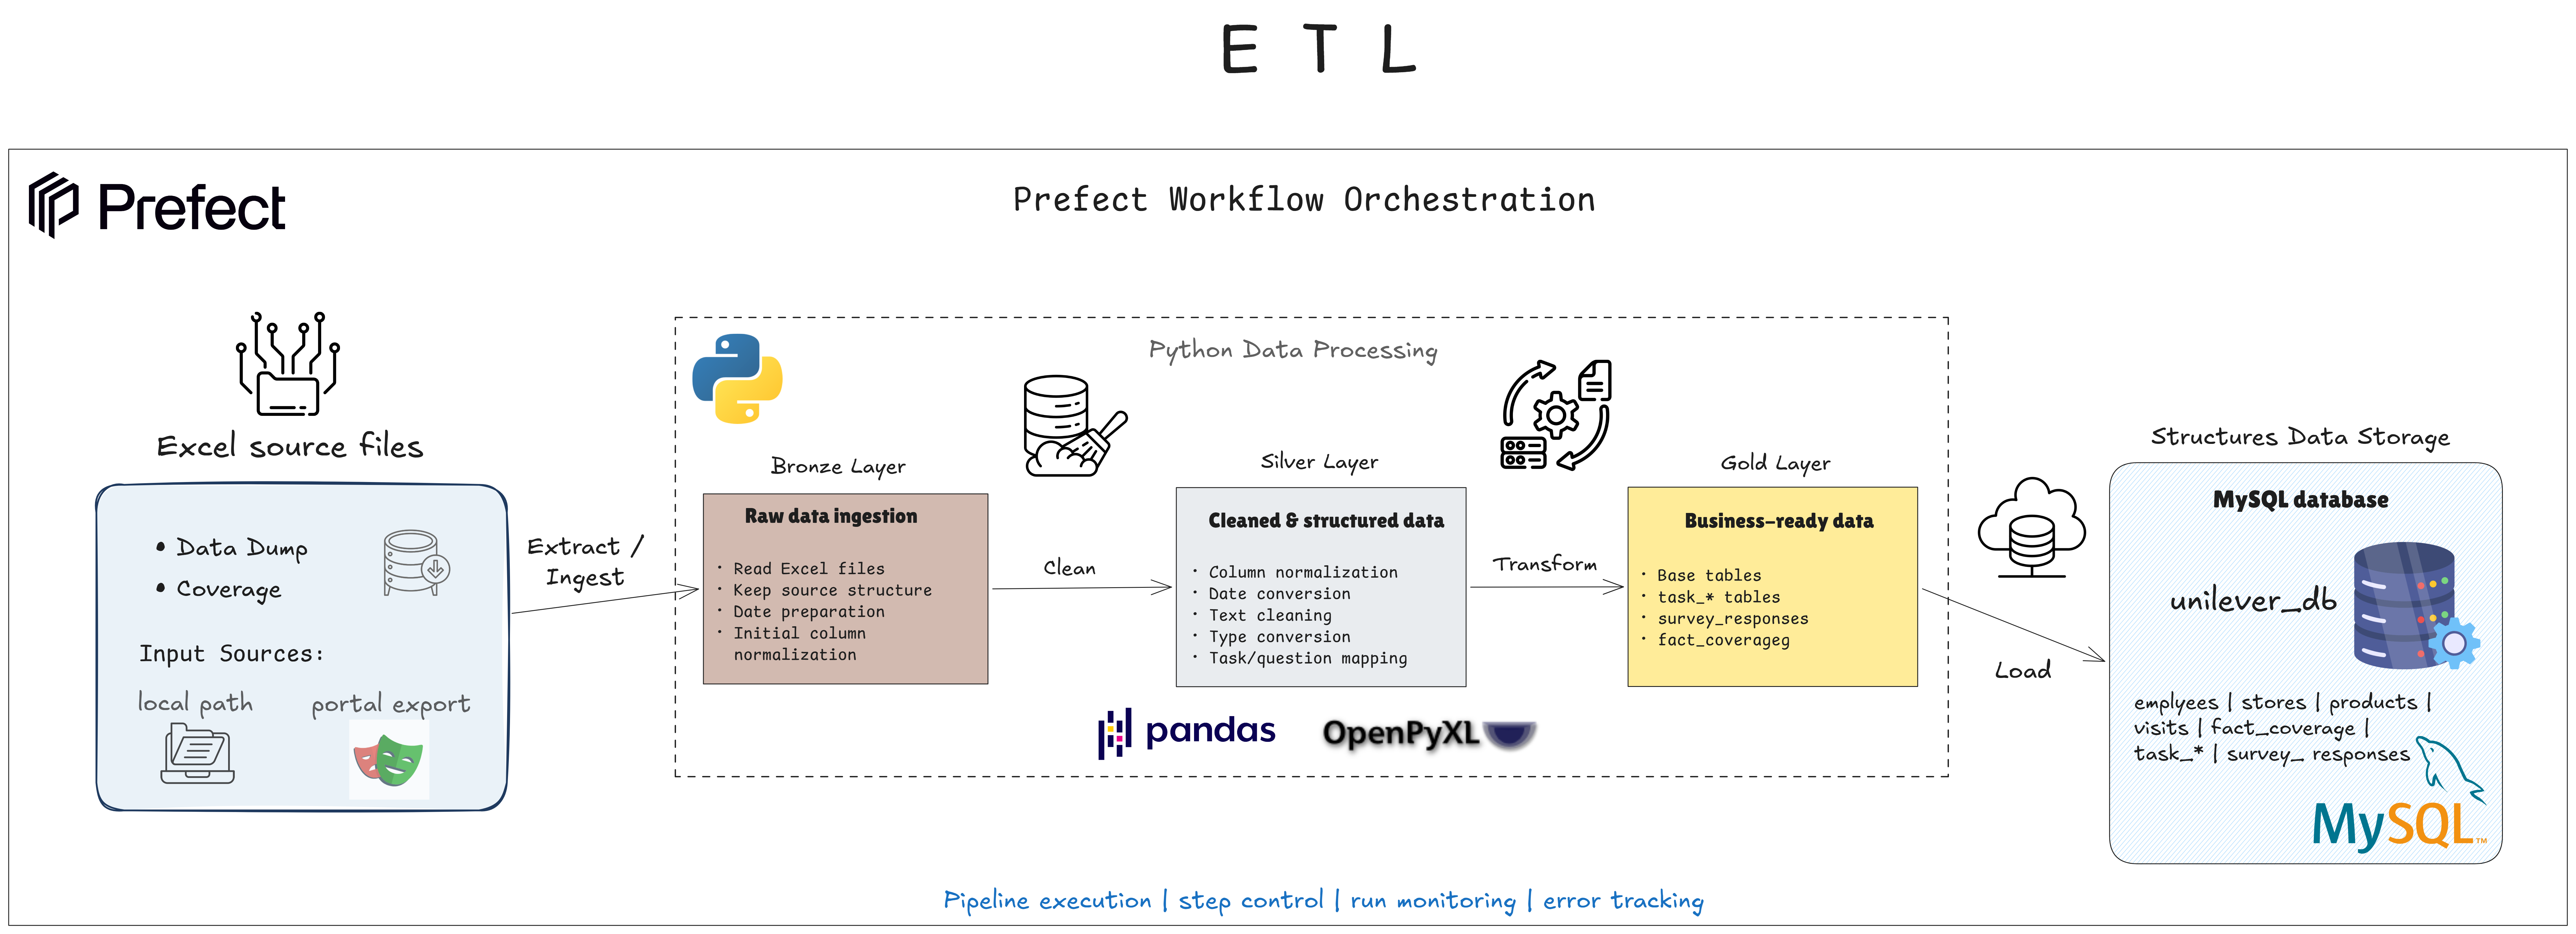
\includegraphics[width=1\textwidth]{figures/etl/ETL.png}
\caption{Flux général du pipeline Data Engineering}
\label{fig:flux_etl}
\end{figure}

Le pipeline part des fichiers sources \textit{Data Dump} et \textit{Coverage}. Les données sont ensuite lues, nettoyées, harmonisées et transformées à l’aide de scripts Python, selon une logique progressive inspirée des couches Bronze, Silver et Gold. Les résultats sont finalement chargés dans MySQL afin d’alimenter les règles de validation, les tableaux de bord et les services backend.

\subsection{Ingestion des fichiers Excel}

L’ingestion constitue la première étape du pipeline Data Engineering. Elle consiste à récupérer les deux fichiers opérationnels nécessaires au traitement : le \textit{Data Dump}, qui contient les réponses détaillées issues des visites terrain, et le \textit{Coverage}, qui fournit une vision opérationnelle des visites planifiées, réalisées, rejetées, déviées ou non effectuées.

Deux modes d’entrée ont été prévus afin de rendre le traitement flexible. Le premier repose sur l’utilisation de fichiers Excel disponibles localement, tandis que le second s’appuie sur l’automatisation de l’export depuis le portail Smollan à l’aide de Playwright \cite{playwright-doc}. Cette double possibilité permet de traiter aussi bien des fichiers déjà téléchargés que des exports récupérés directement depuis le portail.

Le traitement des fichiers repose ensuite sur Python, pandas et openpyxl, utilisés pour lire, nettoyer et transformer les données tabulaires issues des exports opérationnels \cite{python-doc,pandas-doc,openpyxl-doc}.

\subsubsection{Lancement du pipeline}

Le pipeline est lancé depuis le terminal à partir de l’environnement virtuel du projet. Cette commande permet d’exécuter le module principal \textit{main.py}, situé dans le dossier \textit{data-engineering}, puis d’ouvrir l’interface de sélection des fichiers.

\begin{figure}[H]
\centering

\includegraphics[width=0.82\textwidth]{figures/etl/commande_lancement_pipeline.png}
\caption{Commande de lancement du pipeline ETL}
\label{fig:commande_lancement_pipeline}
\end{figure}

La figure \ref{fig:commande_lancement_pipeline} présente la commande utilisée comme point d’entrée du pipeline avant la sélection des fichiers \textit{Data Dump} et \textit{Coverage}.

\subsubsection{Interface de sélection des fichiers}

Après le lancement de la commande, une interface graphique permet de configurer l’exécution du pipeline. Elle permet de sélectionner les fichiers \textit{Data Dump} et \textit{Coverage}, puis de choisir le mode d’entrée : extraction depuis le portail Smollan ou chargement de fichiers Excel disponibles localement.

\begin{figure}[H]
\centering
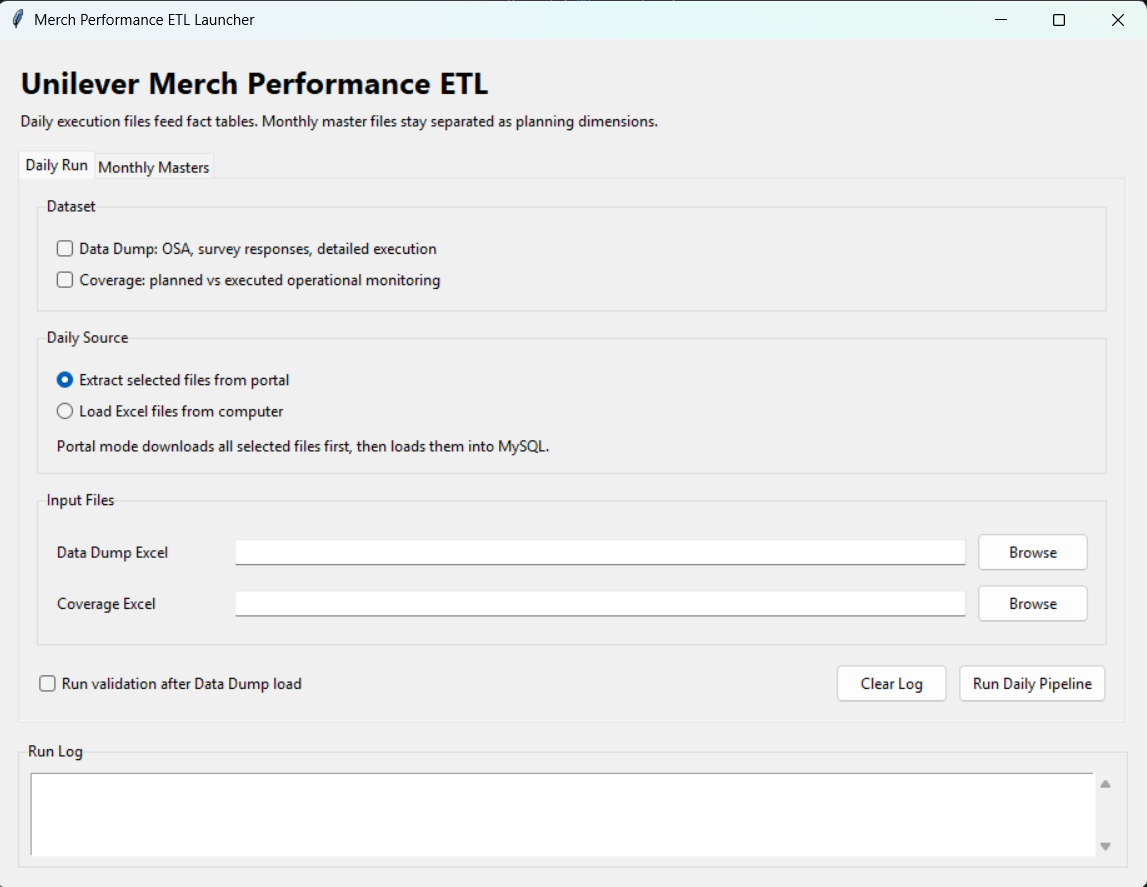
\includegraphics[width=0.7\textwidth]{figures/etl/etl_launcher_interface.png}
\caption{Interface de sélection des fichiers du pipeline ETL}
\label{fig:etl_launcher_interface}
\end{figure}

La figure \ref{fig:etl_launcher_interface} montre que l’interface regroupe les principales options nécessaires au lancement du traitement. Elle permet également d’intégrer l’exécution des règles de validation après le chargement du \textit{Data Dump}.

\subsubsection{Configuration de l’environnement}

La configuration du pipeline repose sur un fichier \textit{.env}. Ce fichier regroupe les paramètres nécessaires à la connexion MySQL, à l’accès au portail Smollan et à l’organisation des répertoires utilisés par le pipeline. Les informations sensibles, comme les identifiants et les mots de passe, sont anonymisées dans le rapport.

\begin{figure}[H]
\centering
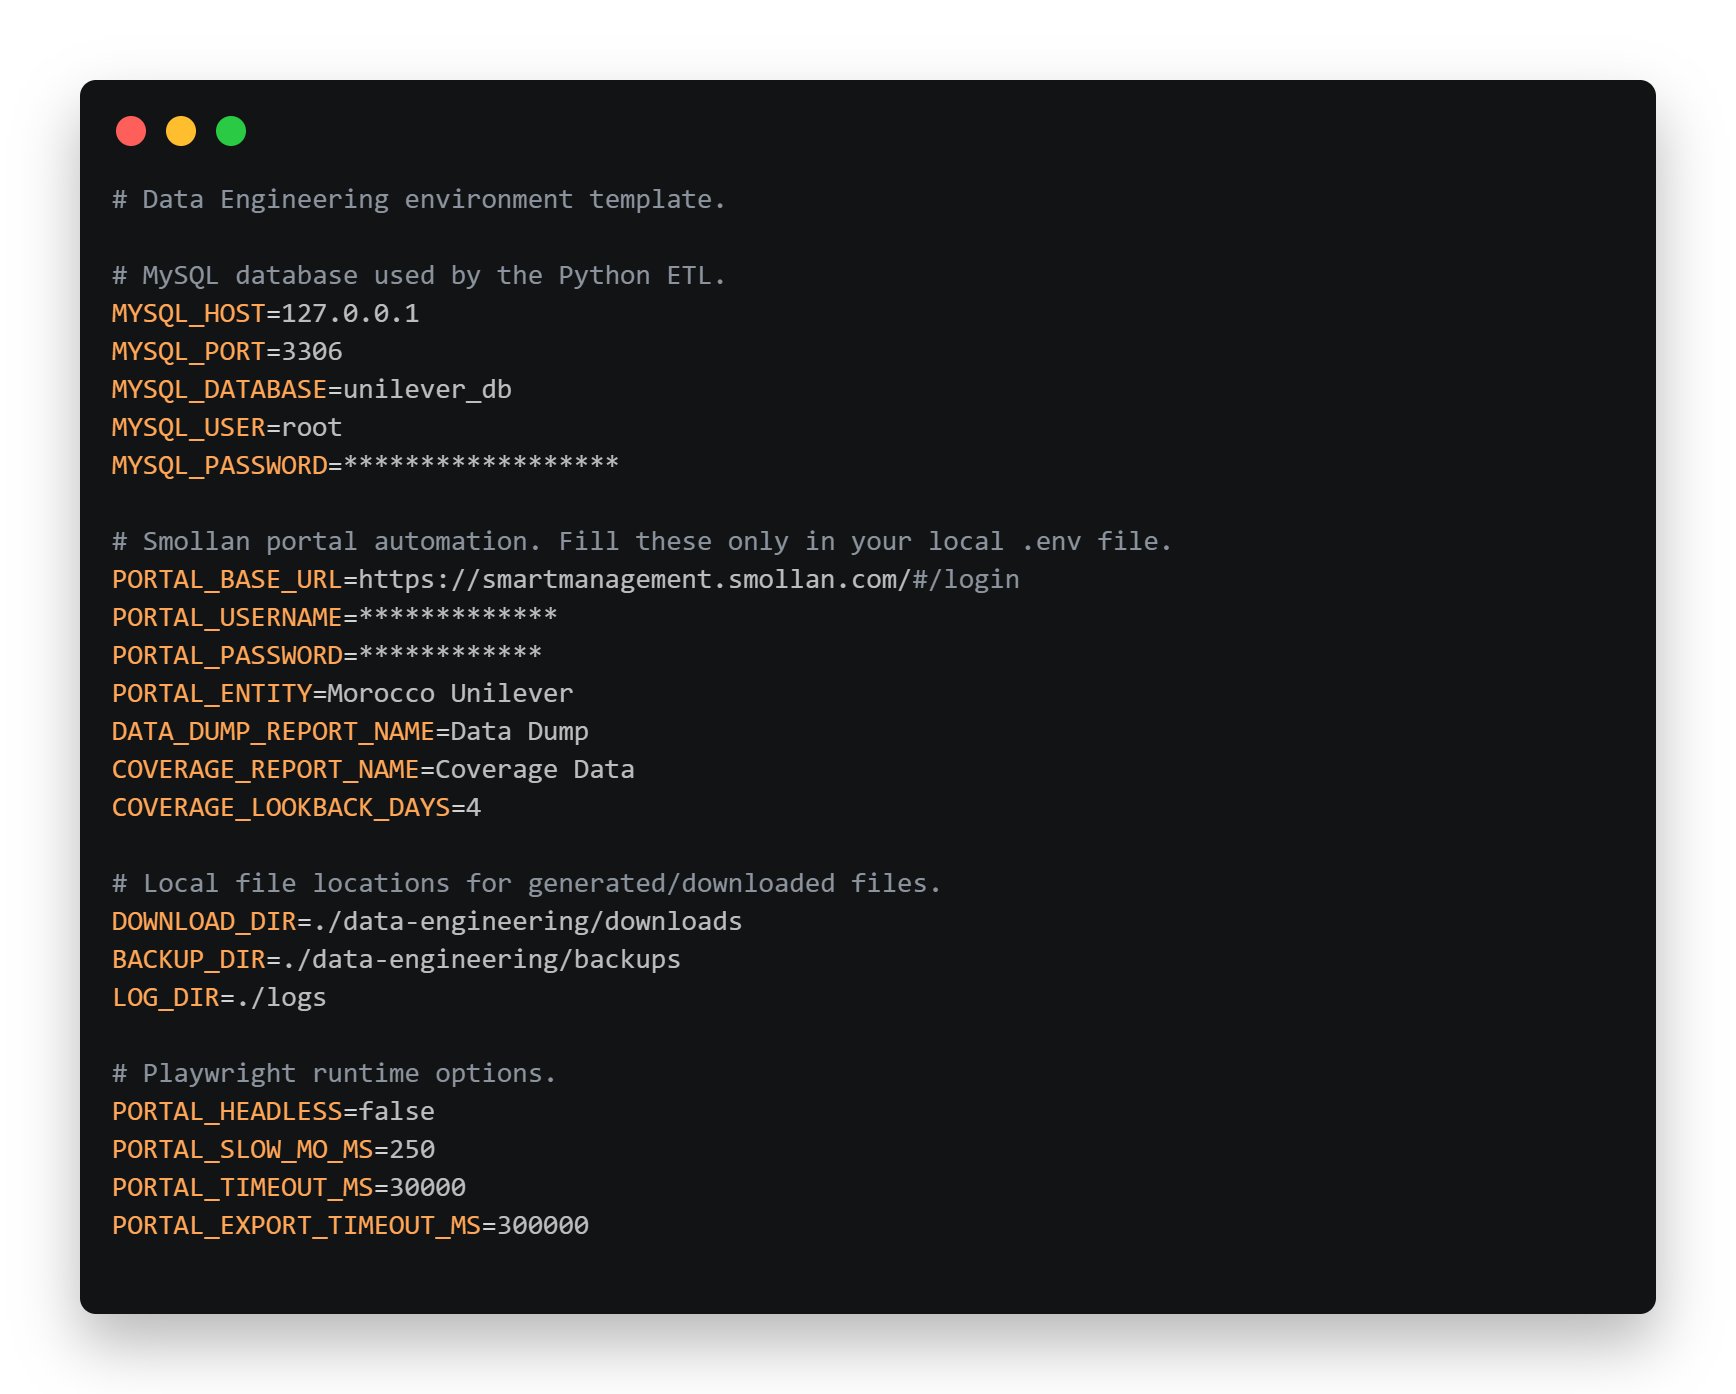
\includegraphics[width=0.62\textwidth]{figures/etl/config_env_pipeline.png}
\caption{Exemple anonymisé de configuration de l’environnement}
\label{fig:config_env_pipeline}
\end{figure}

La figure \ref{fig:config_env_pipeline} présente les principaux paramètres utilisés : informations de connexion à la base \dbtable{unilever\_db}, paramètres d’accès au portail, rapports à extraire et chemins de stockage des fichiers et des logs.

\subsubsection{Orchestration et suivi d’exécution avec Prefect}

L’exécution du pipeline est orchestrée à l’aide de Prefect afin de structurer les différentes étapes du traitement et de faciliter leur suivi \cite{prefect-doc}. Dans la solution, Prefect permet de regrouper les traitements dans un flux principal, tout en séparant les grandes phases fonctionnelles du pipeline.

La structure retenue repose sur un flux principal intitulé \textit{Merch Performance Daily ETL Orchestration}. Ce flux est organisé en sous-flux afin de distinguer les principales étapes : vérifications préalables, acquisition des fichiers, traitement du \textit{Data Dump}, exécution des règles de validation, traitement du \textit{Coverage} et synthèse finale.

\begin{figure}[H]
\centering
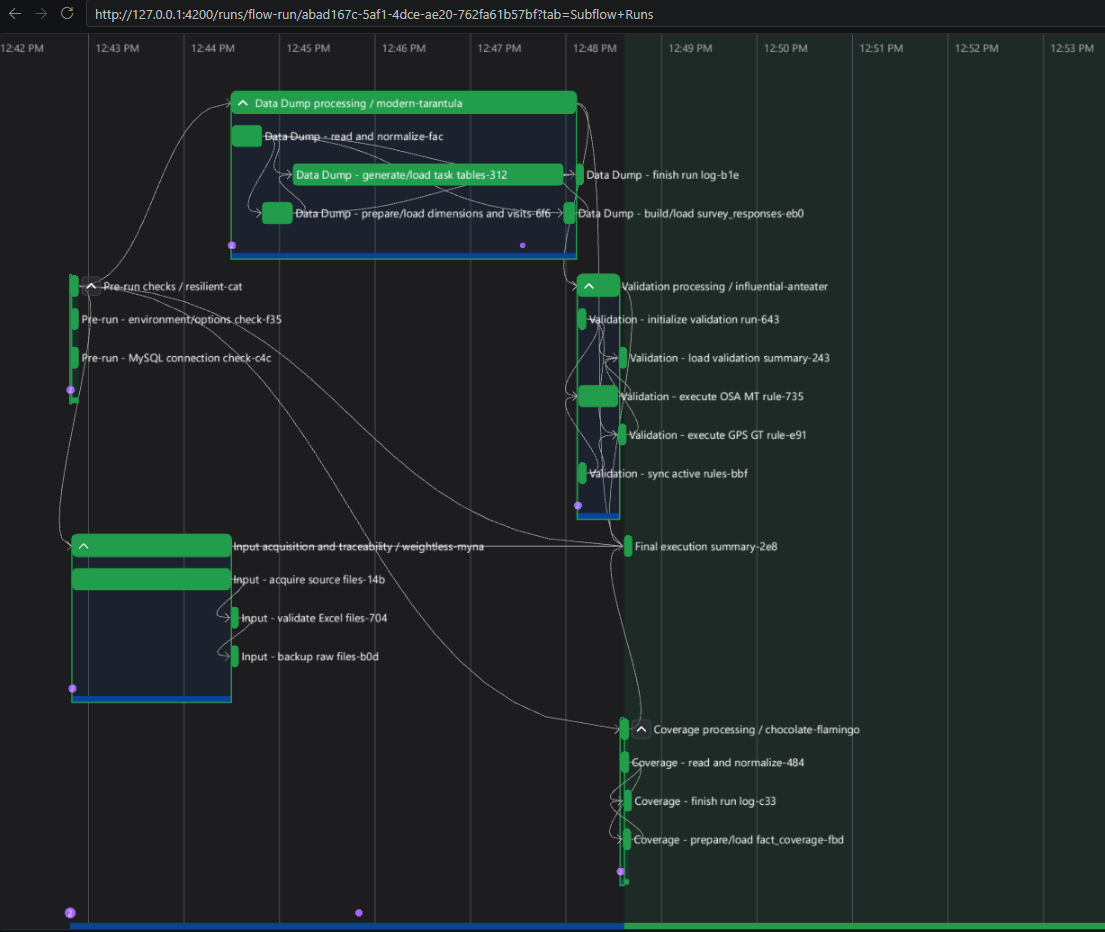
\includegraphics[width=0.97\textwidth]{figures/etl/prefect_parent_flow.png}
\caption{Vue globale de l’orchestration du pipeline dans Prefect}
\label{fig:prefect_parent_flow}
\end{figure}

La figure \ref{fig:prefect_parent_flow} illustre la relation entre le flux principal et les sous-flux fonctionnels. Cette organisation permet de conserver une lecture claire du pipeline, sans afficher toutes les opérations internes comme des tâches indépendantes. Les opérations de bas niveau, telles que les transformations de données, les insertions SQL ou les requêtes propres aux règles de validation, restent encapsulées dans des fonctions Python internes.

Ainsi, Prefect apporte une meilleure structuration par rapport à l’exécution d’un script unique. Les preuves d’exécution du pipeline, les runs terminés et les journaux détaillés seront présentés dans le chapitre consacré aux tests et aux résultats.

\subsection{Traitement du fichier Data Dump}

Le fichier \textit{Data Dump} constitue la source principale des réponses terrain. Il contient les informations issues des visites réalisées dans l’application Smart 3, notamment les données liées aux merchandisers, aux magasins, aux produits, aux tâches, aux questions et aux réponses saisies.

Le traitement de ce fichier consiste à transformer les lignes brutes en tables structurées dans MySQL. Deux exemples représentatifs sont retenus pour illustrer cette logique : les réponses OSA et les données SOS. Ces cas montrent que le pipeline adapte la structure SQL selon la nature métier de chaque tâche.

\begin{figure}[H]
\centering
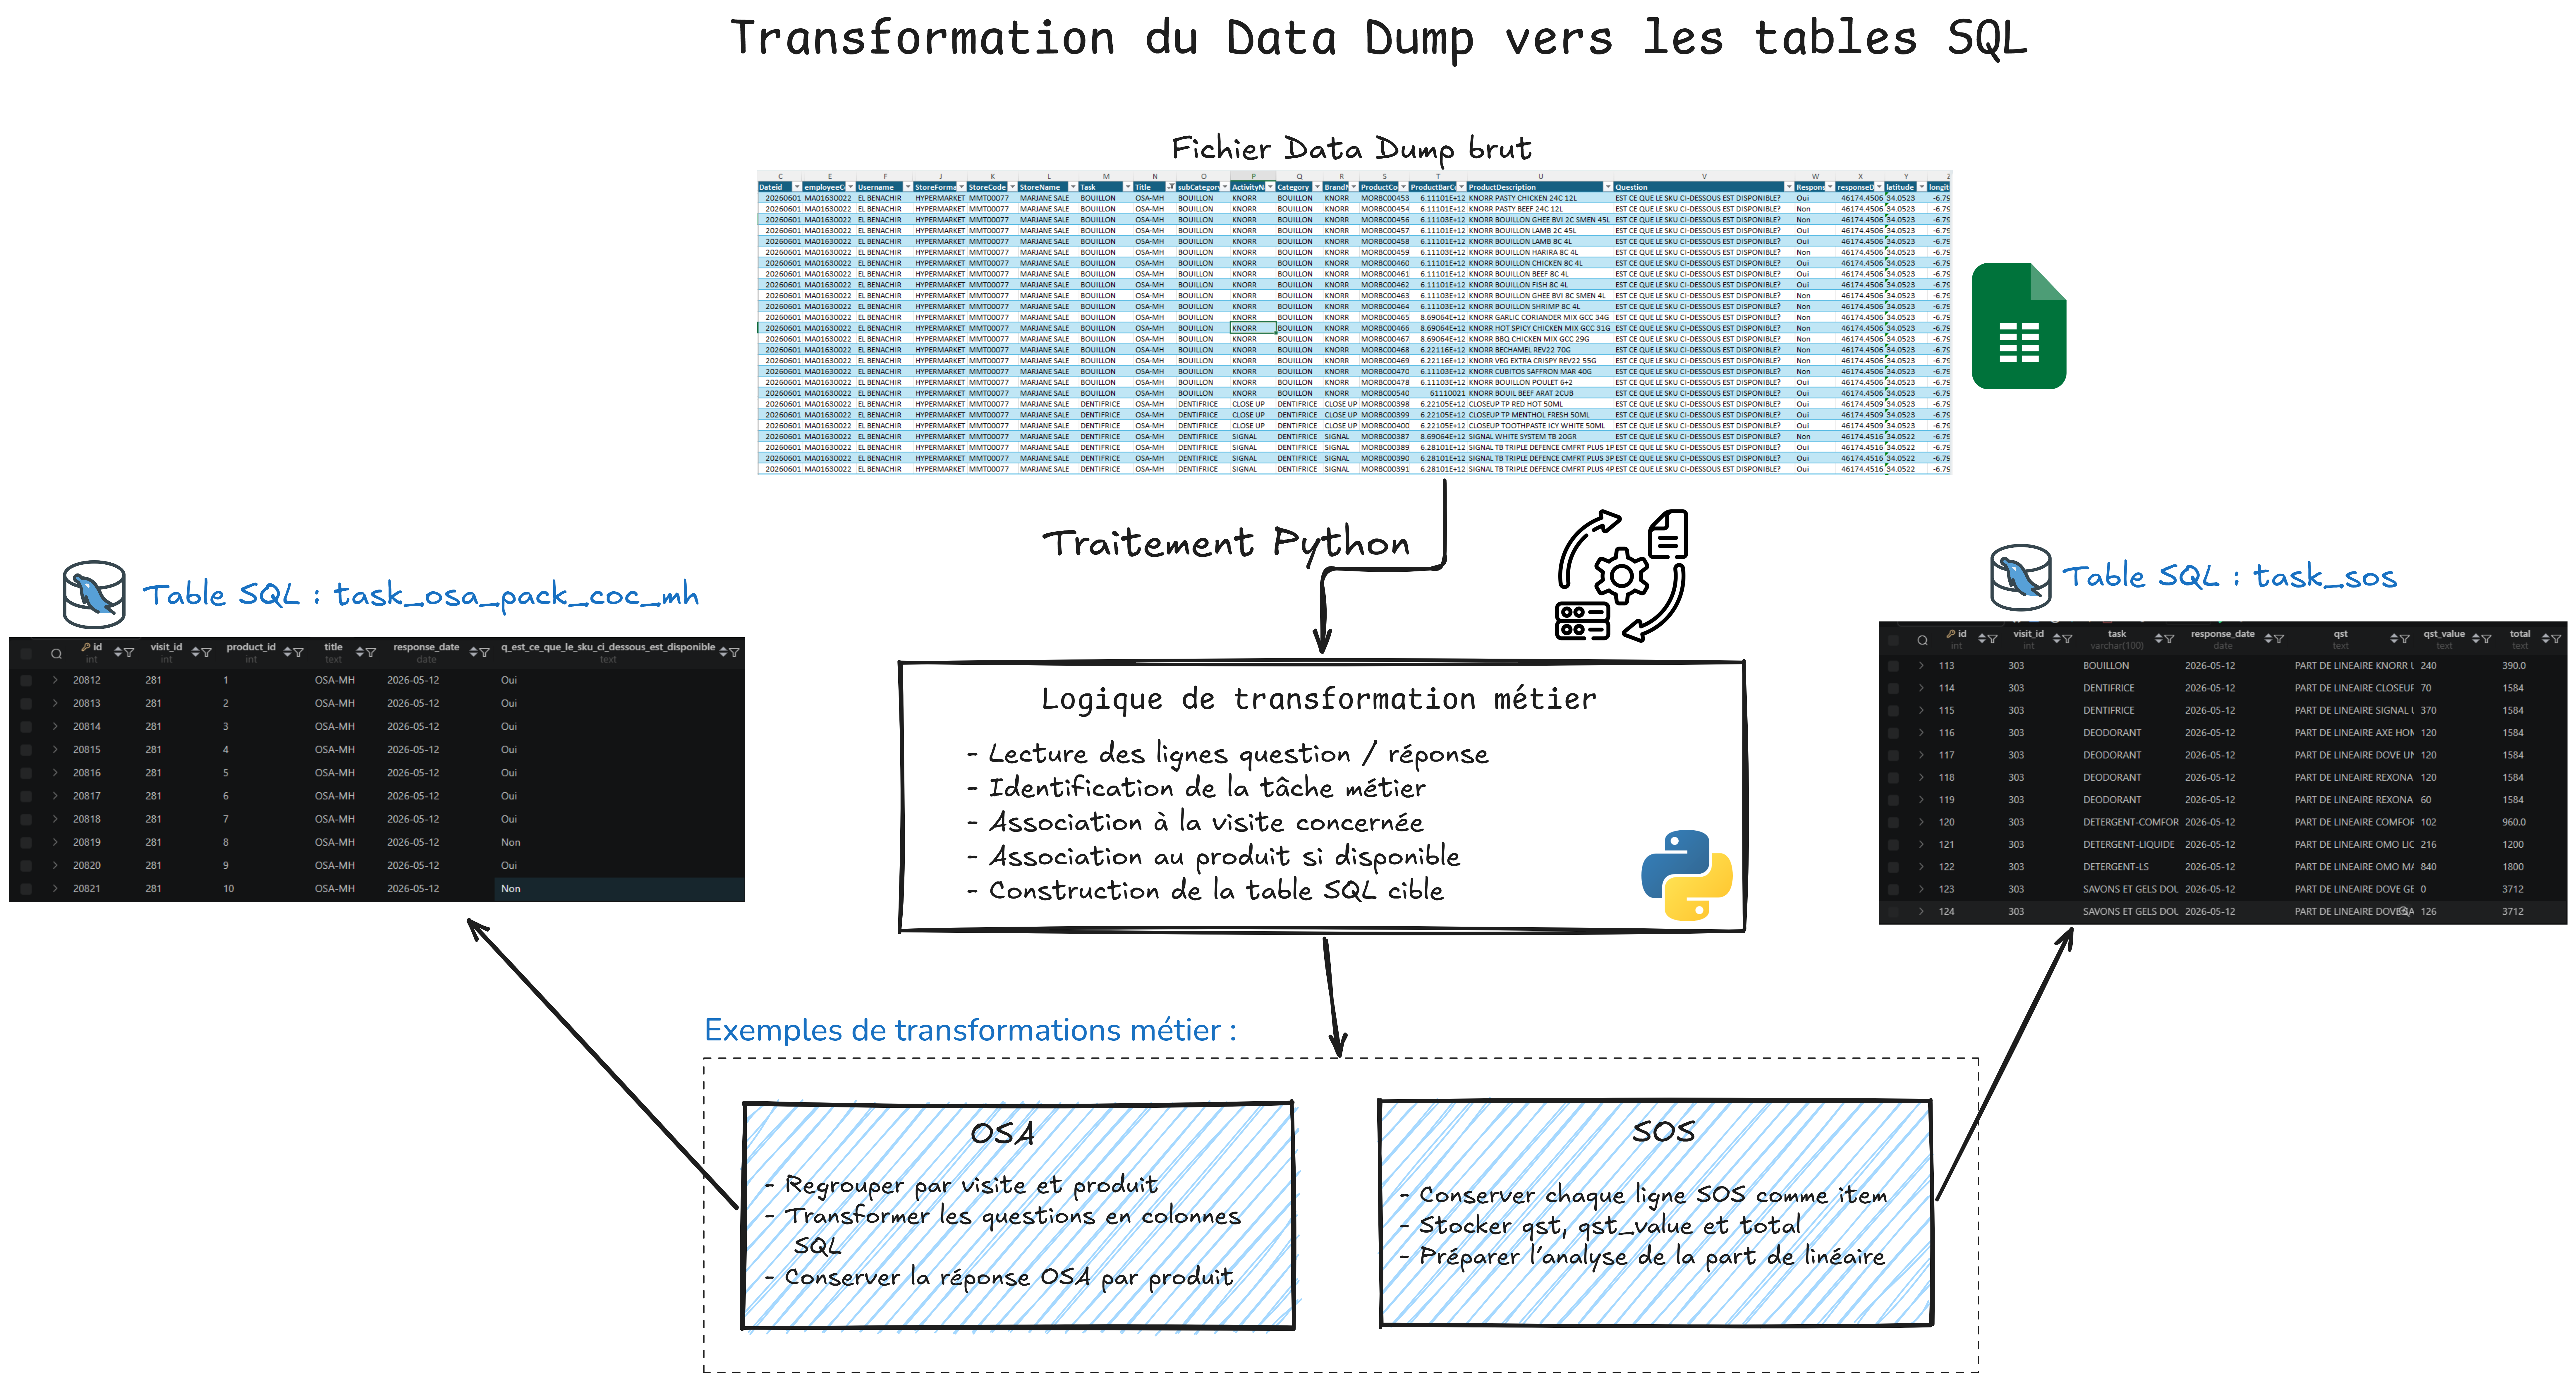
\includegraphics[width=0.90\textwidth]{figures/etl/data_dump_to_sql_transformation.png}
\caption{Transformation du Data Dump vers les tables SQL : exemples OSA et SOS}
\label{fig:data_dump_to_sql_transformation}
\end{figure}

\subsubsection{Principe général de transformation}

Le traitement commence par la lecture des lignes du \textit{Data Dump}. Chaque ligne correspond à une réponse terrain associée à une tâche, une question et une valeur saisie. Le pipeline identifie la tâche concernée, rattache la réponse à la visite correspondante et, lorsque cela est possible, l’associe au produit concerné.
\newpage
Cette étape permet de passer d’une logique Excel orientée lignes de réponses vers une logique SQL structurée. Les champs de liaison reposent principalement sur la date, le code merchandiser et le code magasin, tandis que le code produit permet d’enrichir certaines tâches liées à la disponibilité produit.

\begin{table}[H]
\centering
\caption{Comparaison des transformations appliquées aux cas OSA et SOS}
\label{tab:comparison_osa_sos}
\renewcommand{\arraystretch}{1.25}
\small
\begin{tabular}{
|p{3.2cm}
|p{5.2cm}
|p{5.2cm}|
}
\hline
\textbf{Aspect} & \textbf{Cas OSA} & \textbf{Cas SOS} \\
\hline
Nature des données
& Disponibilité produit par visite et SKU.
& Part de linéaire par visite et item. \\
\hline
Logique de transformation
& Pivot : les questions deviennent des colonnes.
& Structure verticale : une mesure par ligne. \\
\hline
Table cible
& \dbtable{task\_osa\_pack\_coc\_mh}
& \dbtable{task\_sos} \\
\hline
Granularité
& Une ligne par visite et produit.
& Une ligne par item SOS relevé. \\
\hline
Utilité analytique
& Analyse OSA et contrôles de disponibilité.
& Agrégation SOS et visibilité en rayon. \\
\hline
\end{tabular}
\end{table}

Cette comparaison montre que le pipeline adapte la structure SQL selon la nature métier des données. Les réponses OSA sont organisées pour faciliter l’analyse par visite et par produit, tandis que les données SOS conservent une structure verticale afin de préserver la logique de mesure de la part de linéaire.

\subsubsection{Sorties générées et fiabilisation du rechargement}

À partir du fichier \textit{Data Dump}, le pipeline alimente plusieurs familles de tables : les tables de référence, les visites, les tables détaillées \dbtable{task\_*} et la table normalisée \dbtable{survey\_responses}. Cette organisation permet de conserver à la fois des tables spécialisées par tâche et une vue transversale des réponses terrain.

Afin de fiabiliser les relances du pipeline, les données détaillées associées aux visites retraitées sont supprimées avant leur réinsertion. Cette logique évite l’accumulation de doublons et garantit que les tables reflètent le dernier fichier traité.

\subsection{Intégration du Coverage et rapprochement avec le Data Dump}

Le fichier \textit{Coverage} constitue la deuxième source principale du pipeline. Contrairement au \textit{Data Dump}, qui contient les réponses détaillées des visites terrain, le \textit{Coverage} apporte une vision opérationnelle de l’exécution : visites planifiées, réalisées, rejetées, déviées ou non effectuées.

Dans la solution, ce fichier est chargé dans la table \dbtable{fact\_coverage}. Cette table conserve le grain opérationnel du fichier source, principalement basé sur la date de visite, le merchandiser et le magasin. Elle permet ainsi de suivre l’état global de l’exécution, y compris les situations où aucune réponse détaillée n’est disponible dans le \textit{Data Dump}.

\subsubsection{Rôle de la table de couverture opérationnelle}

La table \dbtable{fact\_coverage} joue le rôle d’une table de faits opérationnelle. Elle centralise les informations liées au statut des visites, à la couverture, aux rejets, aux déviations, aux non-visites, aux distances GPS, aux temps d’exécution et aux motifs éventuels.

Son rôle est complémentaire à celui des tables issues du \textit{Data Dump}. Le \textit{Data Dump} permet d’analyser le contenu détaillé des visites exécutées, tandis que le \textit{Coverage} permet d’évaluer l’avancement global du plan de visite.

\subsubsection{Rapprochement avec les visites détaillées}

Afin de relier les données opérationnelles du \textit{Coverage} aux visites détaillées issues du \textit{Data Dump}, une vue SQL a été ajoutée : \dbtable{vw\_fact\_coverage\_visit\_match}. Cette vue permet de comparer les lignes de \dbtable{fact\_coverage} avec les visites présentes dans la table \dbtable{visits}, sans modifier la structure des tables existantes.

L’intérêt de cette approche est de conserver toutes les lignes du \textit{Coverage}, y compris les visites non effectuées, rejetées ou planifiées sans données détaillées. Lorsqu’une correspondance existe, la vue expose le \dbtable{visit\_id}. Dans le cas contraire, elle conserve la ligne Coverage avec un statut indiquant l’absence de visite détaillée.

\begin{figure}[H]
    \centering
    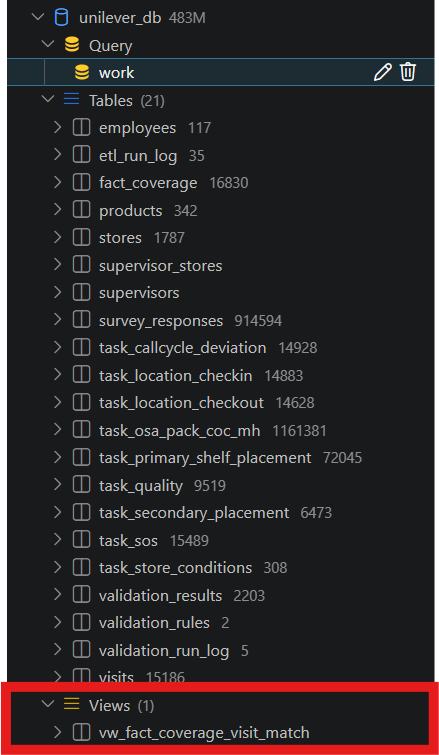
\includegraphics[width=0.37\textwidth]{figures/database/view_coverage_datadump_object.png}
    \caption{Implémentation de la vue SQL de rapprochement dans la base \dbtable{unilever\_db}}
    \label{fig:view_coverage_datadump_object}
\end{figure}

Cette modélisation permet de rapprocher \dbtable{fact\_coverage} et \dbtable{visits} sans imposer de relation physique entre les deux tables. Elle conserve ainsi une lecture complète du \textit{Coverage}, tout en identifiant les visites disposant de réponses détaillées dans le \textit{Data Dump}.

% \subsubsection{Apport dans la solution}

% Cette modélisation renforce la cohérence globale de la solution. Elle évite de forcer une relation physique entre \dbtable{fact\_coverage} et \dbtable{visits}, ce qui aurait pu poser problème pour les visites non effectuées ou rejetées. À la place, la vue SQL propose une lecture contrôlée et réversible, sans imposer de modification directe aux tables existantes ni aux services applicatifs déjà mis en place.

% Elle constitue également une base utile pour les analyses futures, car elle distingue clairement les visites ayant des réponses détaillées de celles qui existent uniquement dans le suivi de couverture. Cette distinction peut ensuite être exploitée dans les tableaux de bord, les contrôles opérationnels ou les interfaces de suivi.

\subsection{Modélisation et chargement dans MySQL}

Après les étapes de préparation et de transformation, les données sont chargées dans une base MySQL nommée \dbtable{unilever\_db}. Cette base constitue le référentiel central de la solution, car elle regroupe les données issues des fichiers \textit{Data Dump} et \textit{Coverage} et les rend exploitables par les règles de validation, les tableaux de bord et les services applicatifs.

Le modèle retenu ne reproduit pas directement la structure des fichiers Excel. Il organise les données selon leur rôle dans la solution : données de référence, visites, réponses terrain, couverture opérationnelle, résultats de validation et journaux d’exécution.

\begin{figure}[H]
    \centering
    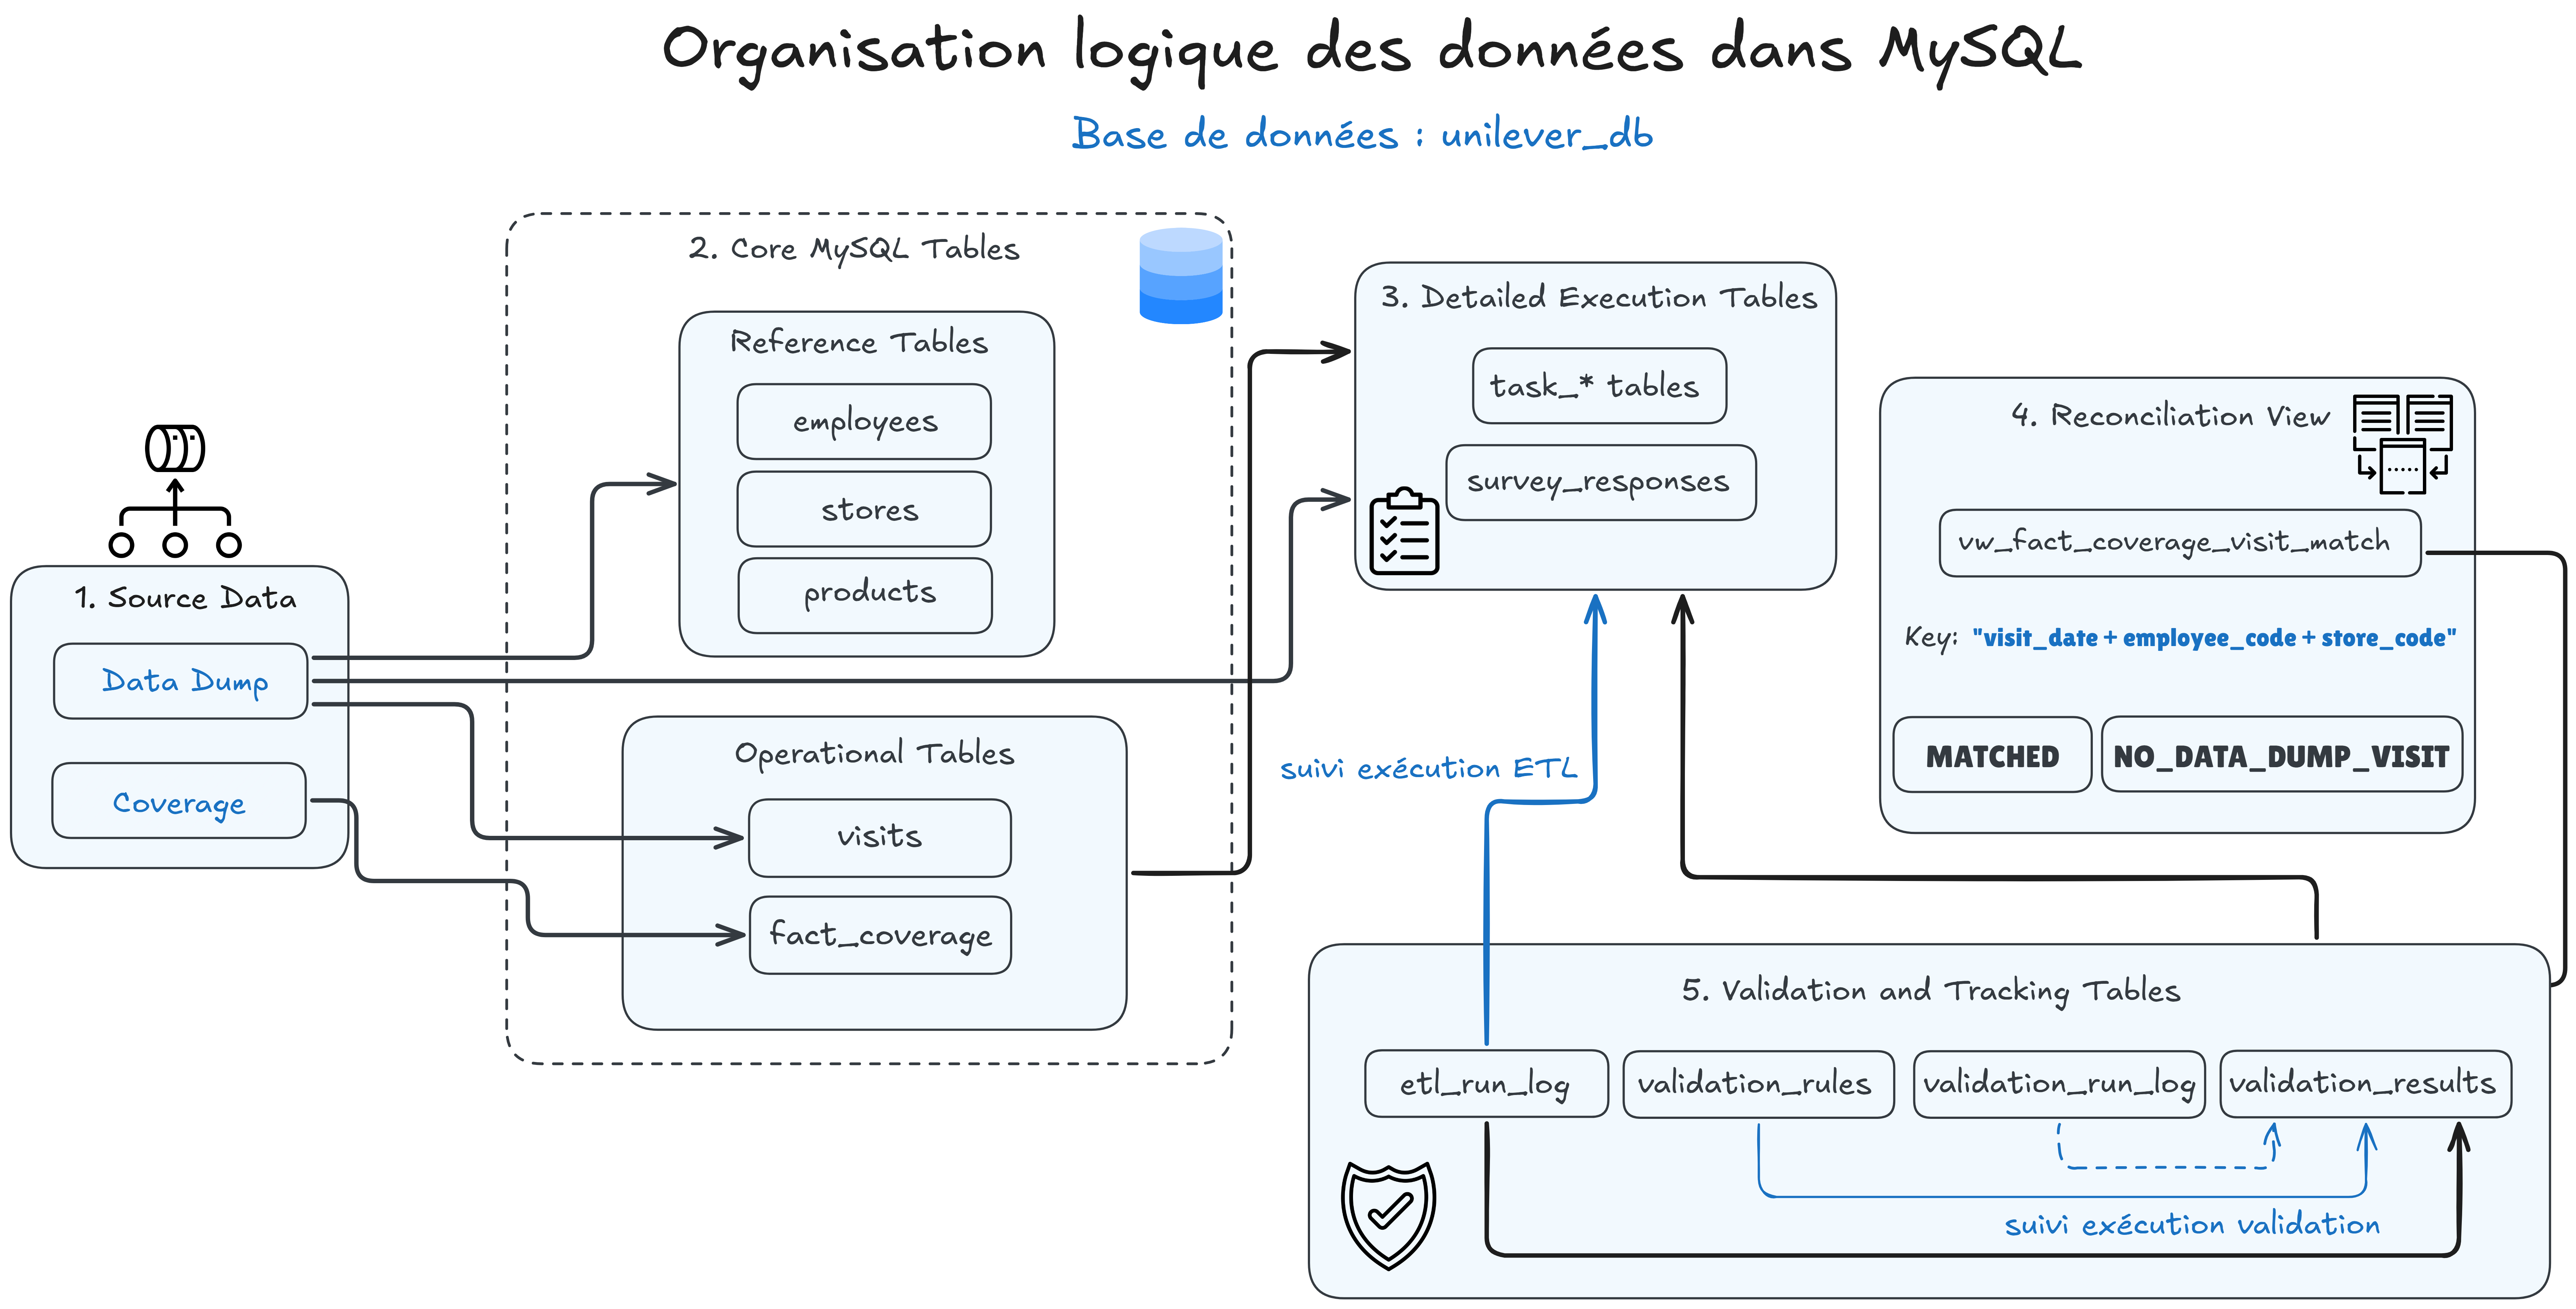
\includegraphics[width=1\textwidth]{figures/database/mysql_logical_model.png}
    \caption{Organisation logique des données dans MySQL}
    \label{fig:mysql_logical_model}
\end{figure}

La figure \ref{fig:mysql_logical_model} présente une vue simplifiée de l’organisation des données dans MySQL. Le \textit{Data Dump} alimente les tables de référence, les visites, les tables de tâches et la table \dbtable{survey\_responses}, tandis que le \textit{Coverage} alimente la table \dbtable{fact\_coverage}. Cette organisation permet de séparer les données stables, opérationnelles et analytiques.

\subsubsection{Stratégie de chargement}

Le chargement des données s’effectue de manière contrôlée afin d’éviter les doublons et de garantir la cohérence des informations insérées. Les tables de référence sont alimentées à partir des codes métier, comme le code employé, le code magasin ou le code produit.

Les visites sont identifiées à partir d’une clé naturelle composée de la date de visite, du merchandiser et du magasin. Pour les réponses détaillées, le pipeline applique une logique de rechargement contrôlé : les anciennes lignes associées aux visites retraitées sont supprimées avant l’insertion des nouvelles données.

\subsubsection{Traçabilité des traitements}

La traçabilité des exécutions est assurée à travers la table \dbtable{etl\_run\_log}. Elle permet de conserver les informations liées aux traitements réalisés, aux fichiers concernés, aux dates d’exécution et à l’état global du chargement.

Cette logique facilite le suivi des traitements et l’analyse en cas d’erreur. Ainsi, le chargement dans MySQL transforme les fichiers Excel traités en un modèle relationnel exploitable par les validations métier, les tableaux de bord et les interfaces de consultation.

\section{Structuration de la base de données}

La base MySQL \dbtable{unilever\_db} est organisée selon le rôle des données dans la solution. Elle regroupe les tables de référence, les tables opérationnelles, les tables détaillées d’exécution, la vue de rapprochement, les tables de validation et les tables de traçabilité.

\begin{figure}[H]
\centering
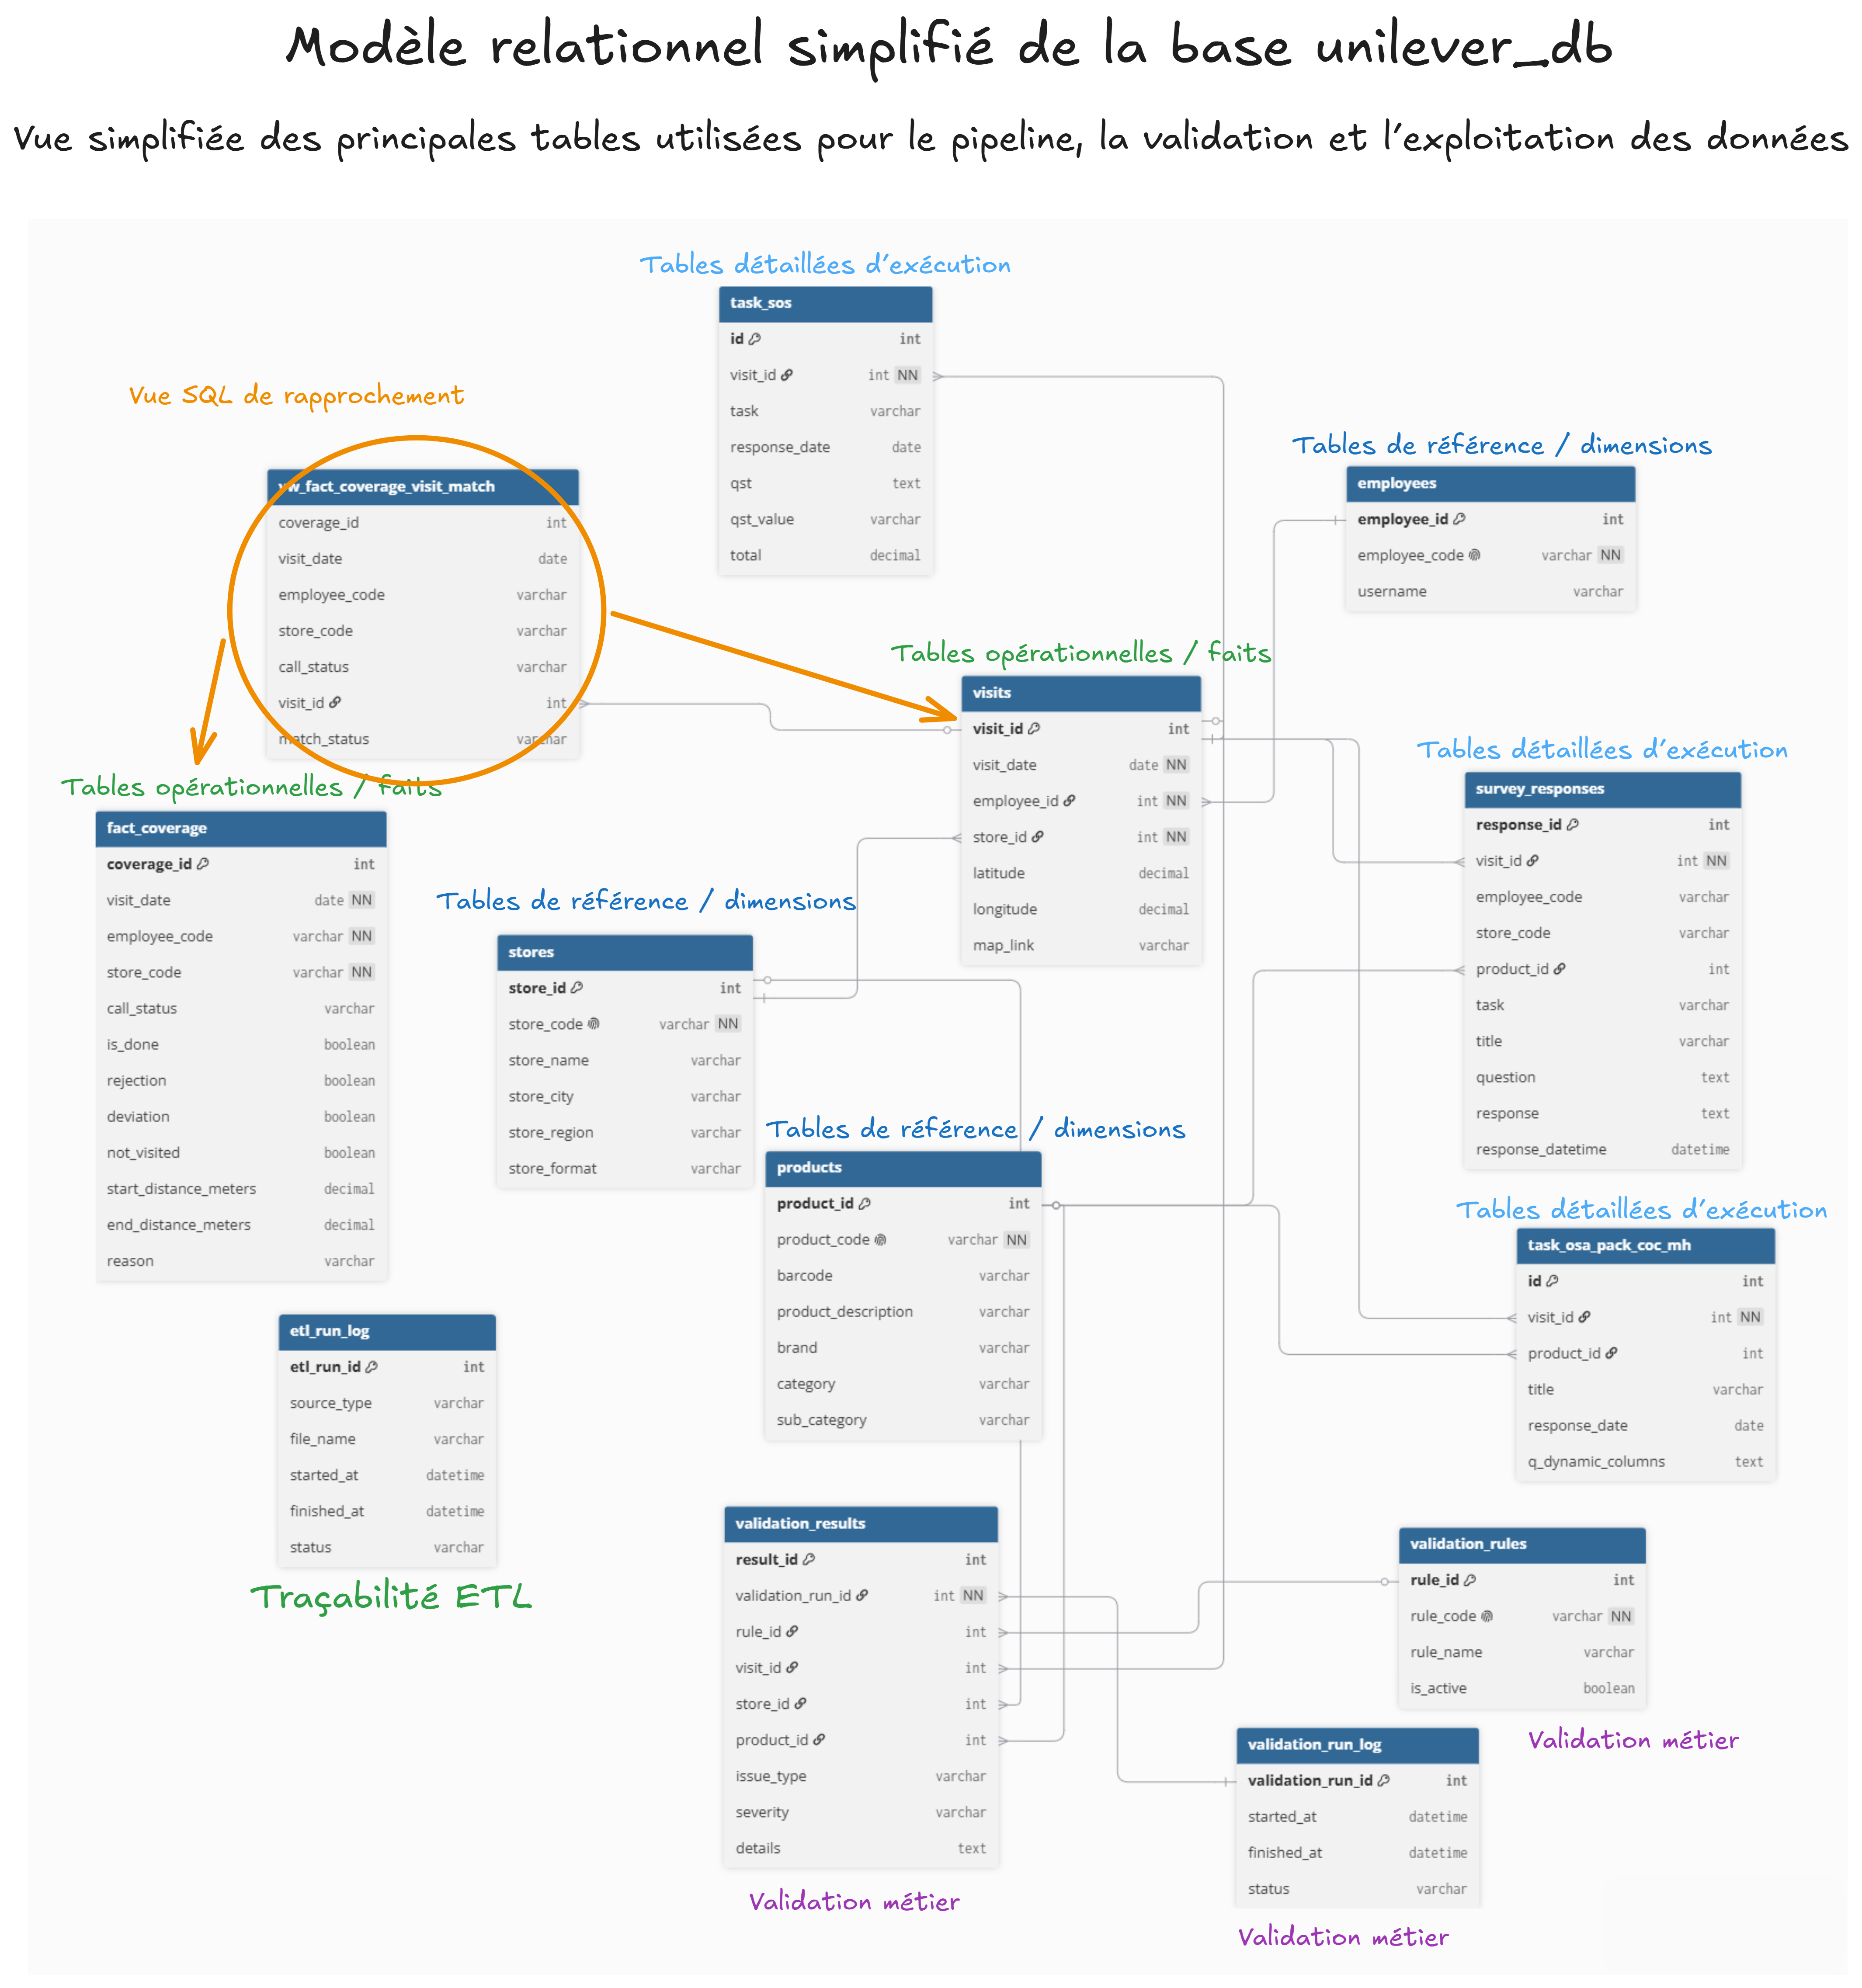
\includegraphics[width=0.90\textwidth]{figures/database/tables_flow.png}
\caption{Modèle relationnel simplifié de la base \dbtable{unilever\_db}}
\label{fig:dbdiagram_simplified_model}
\end{figure}

La figure \ref{fig:dbdiagram_simplified_model} présente une vue simplifiée du modèle relationnel. Les tables \dbtable{employees}, \dbtable{stores} et \dbtable{products} constituent les référentiels métier. Les tables \dbtable{visits} et \dbtable{fact\_coverage} portent les données opérationnelles issues du \textit{Data Dump} et du \textit{Coverage}.

Les tables \dbtable{task\_*} conservent les réponses détaillées selon la nature des tâches terrain, tandis que \dbtable{survey\_responses} fournit une vue normalisée des réponses. Les tables \dbtable{supervisors} et \dbtable{supervisor\_stores} permettent de gérer le périmètre de consultation mobile par superviseur.

Enfin, la vue \dbtable{vw\_fact\_coverage\_visit\_match} assure le rapprochement entre la couverture opérationnelle et les visites détaillées. Les tables \dbtable{validation\_rules}, \dbtable{validation\_run\_log}, \dbtable{validation\_results} et \dbtable{etl\_run\_log} assurent la traçabilité des règles métier, des résultats de validation et des exécutions du pipeline.

\section{Mise en place du moteur de validation}

Après la structuration des données dans MySQL, une couche de validation a été développée afin d’identifier certaines situations nécessitant une vérification opérationnelle. Ce moteur est implémenté en Python et s’appuie sur les données déjà chargées dans la base \dbtable{unilever\_db}, notamment les visites, les magasins, les merchandisers et les réponses terrain.

L’objectif de cette couche n’est pas de remplacer le contrôle humain, mais de préparer une première détection automatique des situations inhabituelles. Les résultats produits par les règles sont stockés dans MySQL afin d’être consultés dans le portail back-office interne.

\subsection{Principe général du moteur de validation}

Le moteur de validation est organisé autour d’un registre de règles Python. Les règles déclarées dans le projet sont synchronisées avec la table \dbtable{validation\_rules}, puis seules les règles actives sont exécutées. Chaque exécution crée une ligne dans \dbtable{validation\_run\_log}, exécute les contrôles métier, insère les situations détectées dans \dbtable{validation\_results}, puis met à jour le statut final de l’exécution.

\begin{figure}[H]
\centering
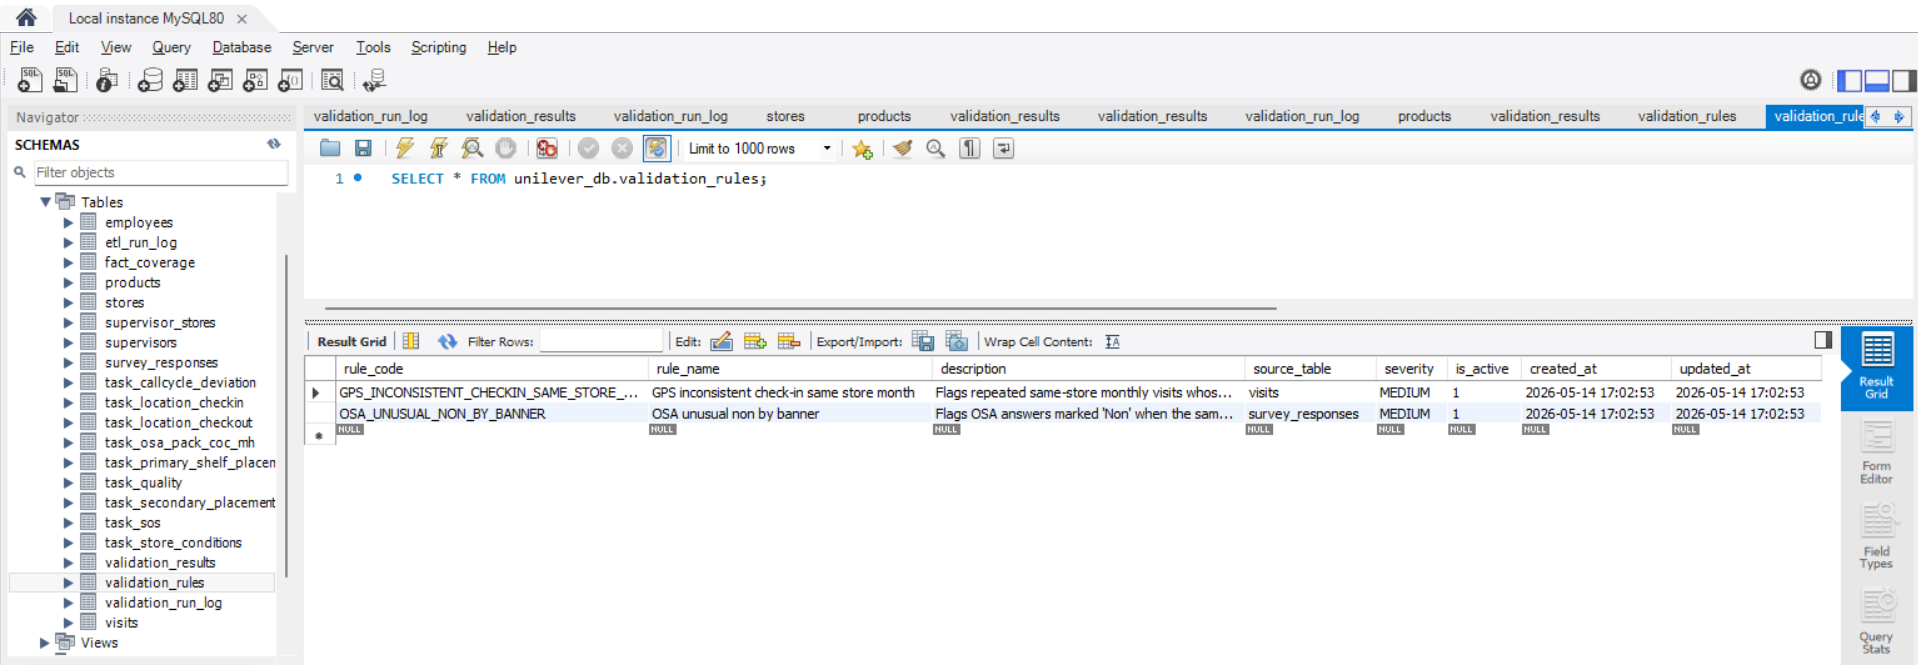
\includegraphics[width=1\textwidth]{figures/validation/validation_rules_mysql1.png}
\caption{Règles de validation enregistrées dans MySQL}
\label{fig:validation_rules_mysql}
\end{figure}

La figure \ref{fig:validation_rules_mysql} montre que les règles de validation sont enregistrées dans la base MySQL. Cette organisation permet de conserver une trace des règles disponibles et de contrôler leur activation avant l’exécution du moteur.

\subsection{Règle OSA appliquée aux formats MT}

La première règle implémentée est la règle \dbtable{OSA\_UNUSUAL\_NON\_BY\_BANNER}. Elle s’applique uniquement aux magasins de type \textit{HYPERMARKET}, \textit{SUPERMARKET LOWER} et \textit{SUPERMARKET UPPER}. Elle exploite les réponses issues de \dbtable{survey\_responses}, croisées avec les tables \dbtable{visits} et \dbtable{stores}.

Cette règle analyse les réponses \textit{Oui} et \textit{Non} liées aux questions contenant le terme \textit{DISPONIBLE}. Elle regroupe les réponses par semaine, produit et question, puis signale les réponses \textit{Non} lorsque le comportement du groupe indique une disponibilité fortement positive. Dans l’implémentation actuelle, la règle exige au moins 10 réponses, au moins 8 réponses \textit{Oui} et un taux de disponibilité supérieur ou égal à 90\%.

\begin{figure}[H]
\centering
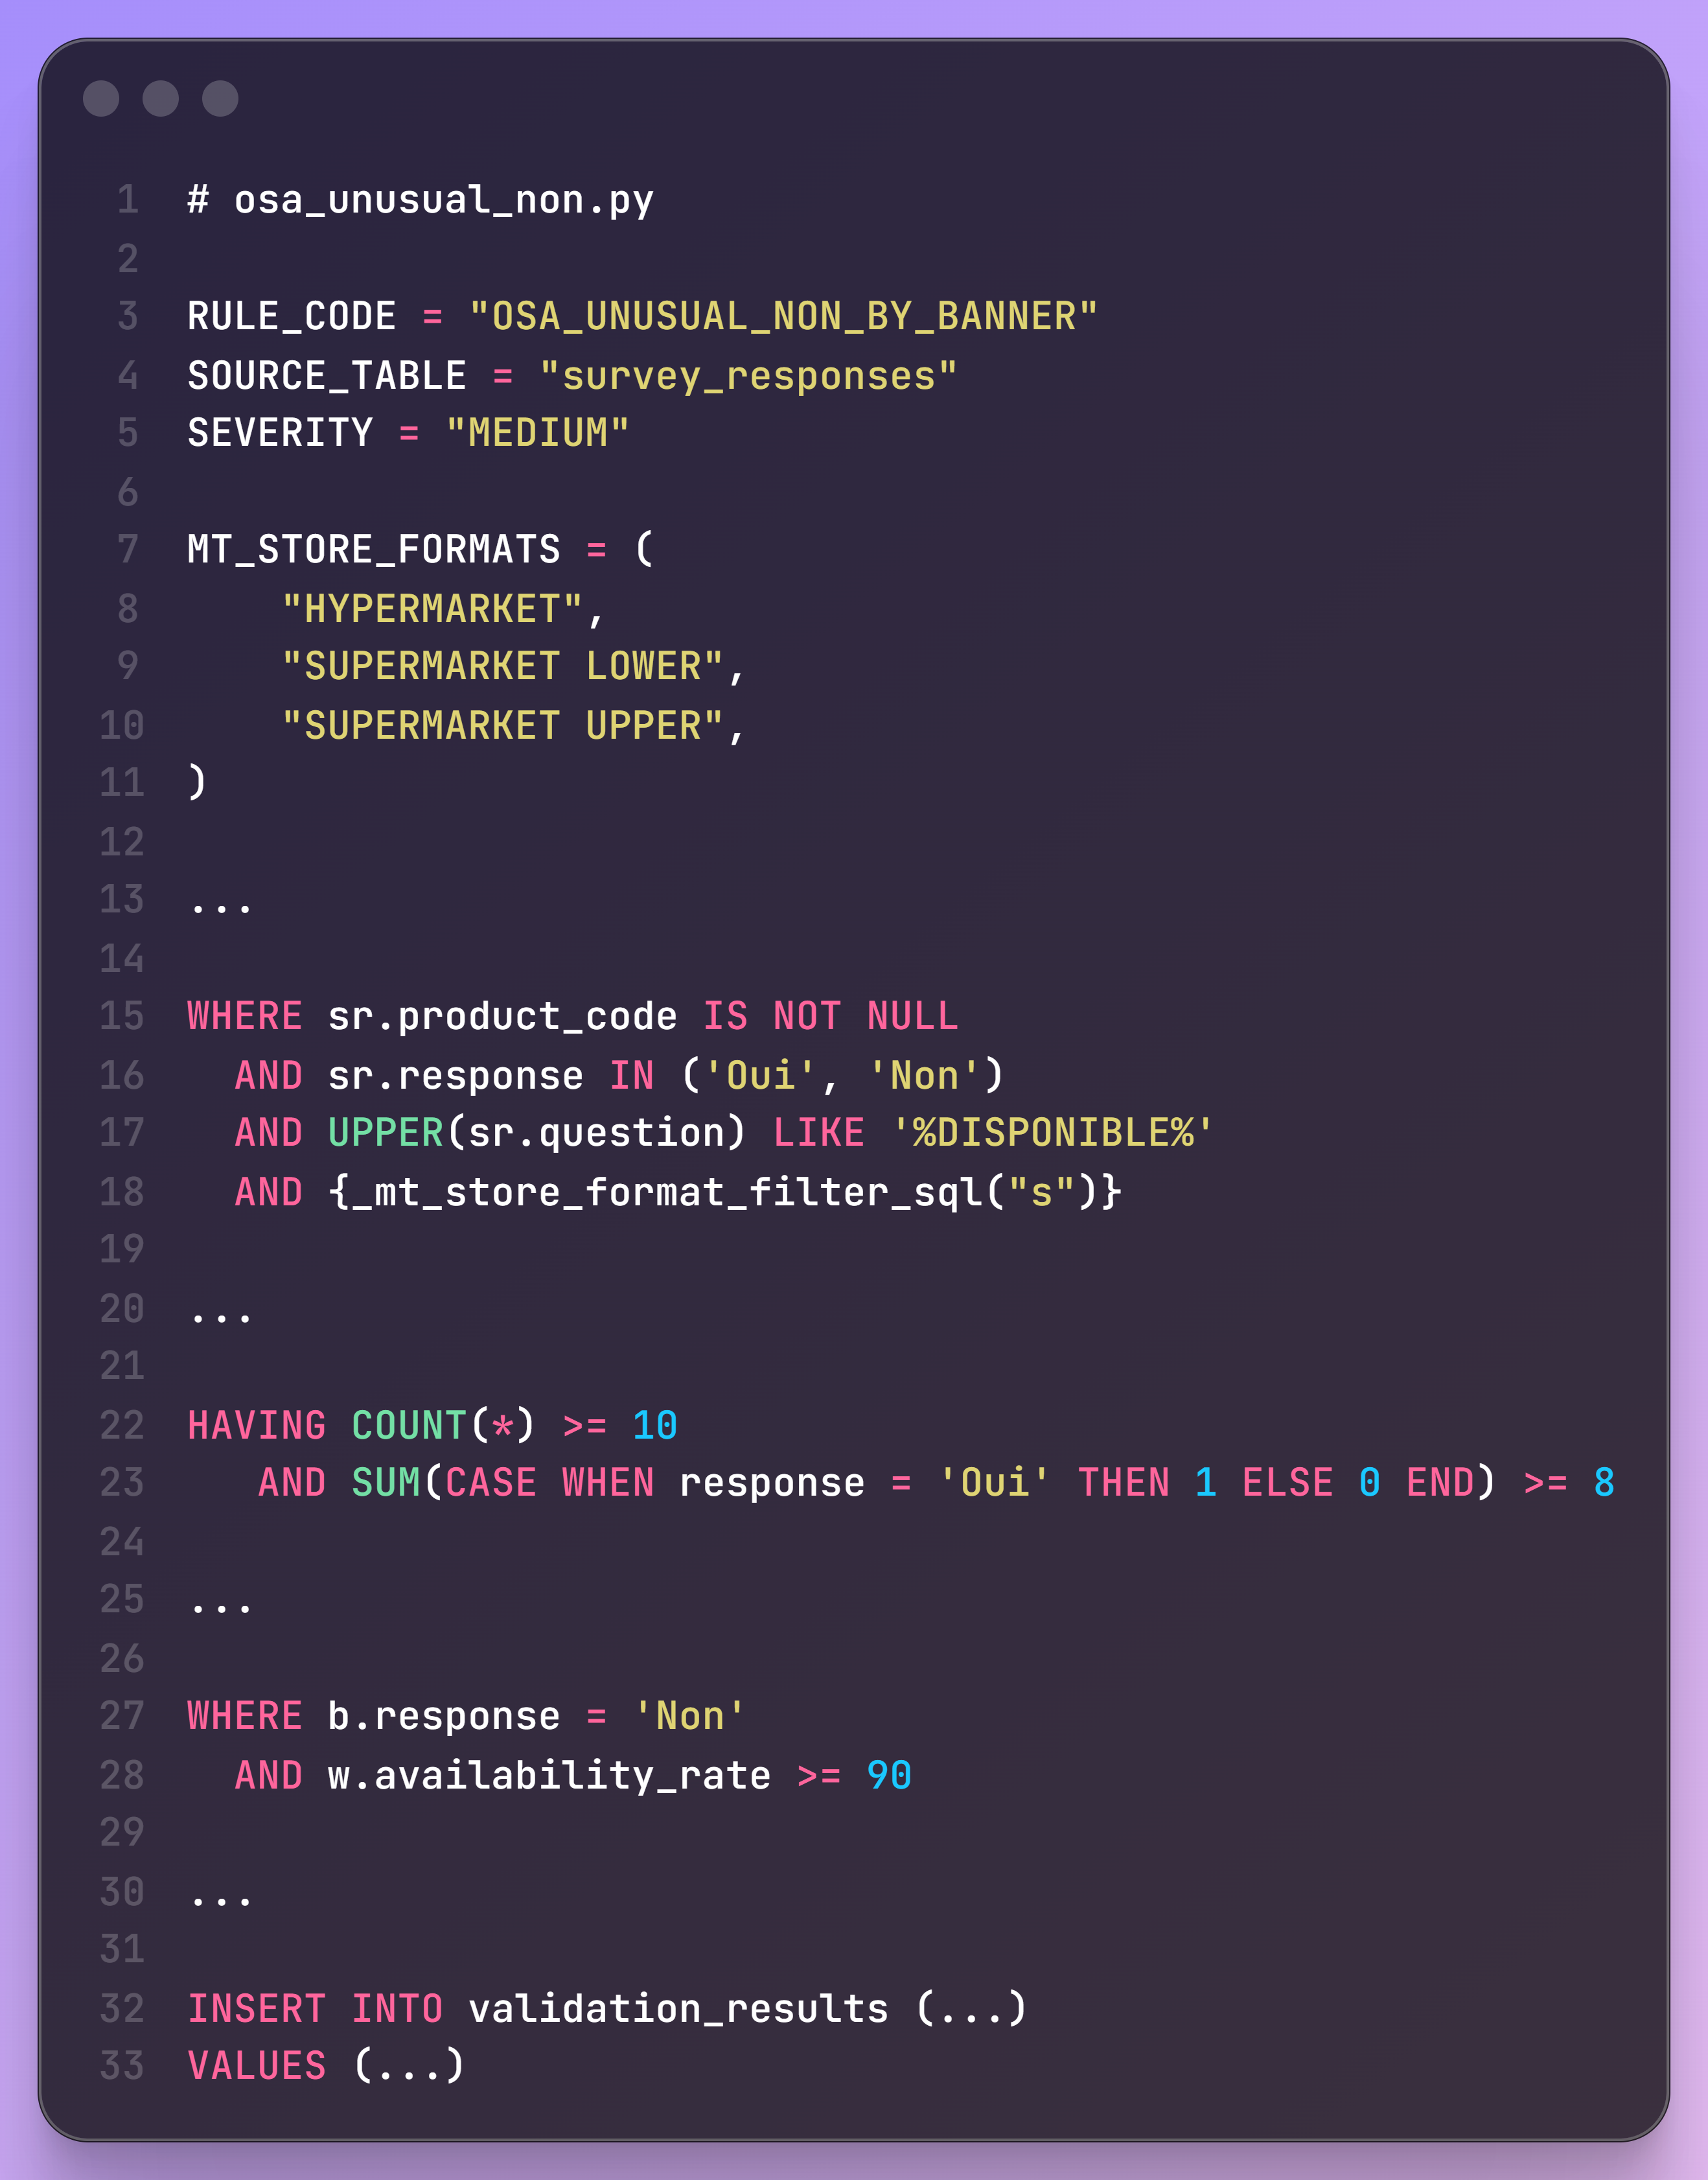
\includegraphics[width=0.60\textwidth]{figures/validation/osa_rule_implementation.png}
\caption{Implémentation de la règle OSA appliquée aux formats MT}
\label{fig:osa_rule_implementation}
\end{figure}

La figure \ref{fig:osa_rule_implementation} présente un extrait du code de la règle OSA. Elle met en évidence le périmètre MT, les filtres appliqués sur les réponses terrain, les seuils de détection et l’insertion des situations détectées dans la table \dbtable{validation\_results}.

\subsection{Règle GPS appliquée aux formats GT}

La deuxième règle implémentée est la règle \dbtable{GPS\_INCONSISTENT\_CHECKIN}. Elle s’applique uniquement aux magasins de type \textit{GROCERY} et \textit{CASH AND CARRY}. Elle repose principalement sur les coordonnées GPS enregistrées dans la table \dbtable{visits}.

Les visites sont regroupées par merchandiser, magasin, année et mois. Pour chaque groupe contenant au moins trois visites, le moteur calcule une position GPS de référence à partir des coordonnées médianes. La distance entre chaque visite et cette position est ensuite calculée. Une situation est détectée lorsque cette distance dépasse 1000 mètres. La sévérité devient \textit{HIGH} lorsque la distance atteint au moins 2000 mètres.

\begin{figure}[H]
\centering
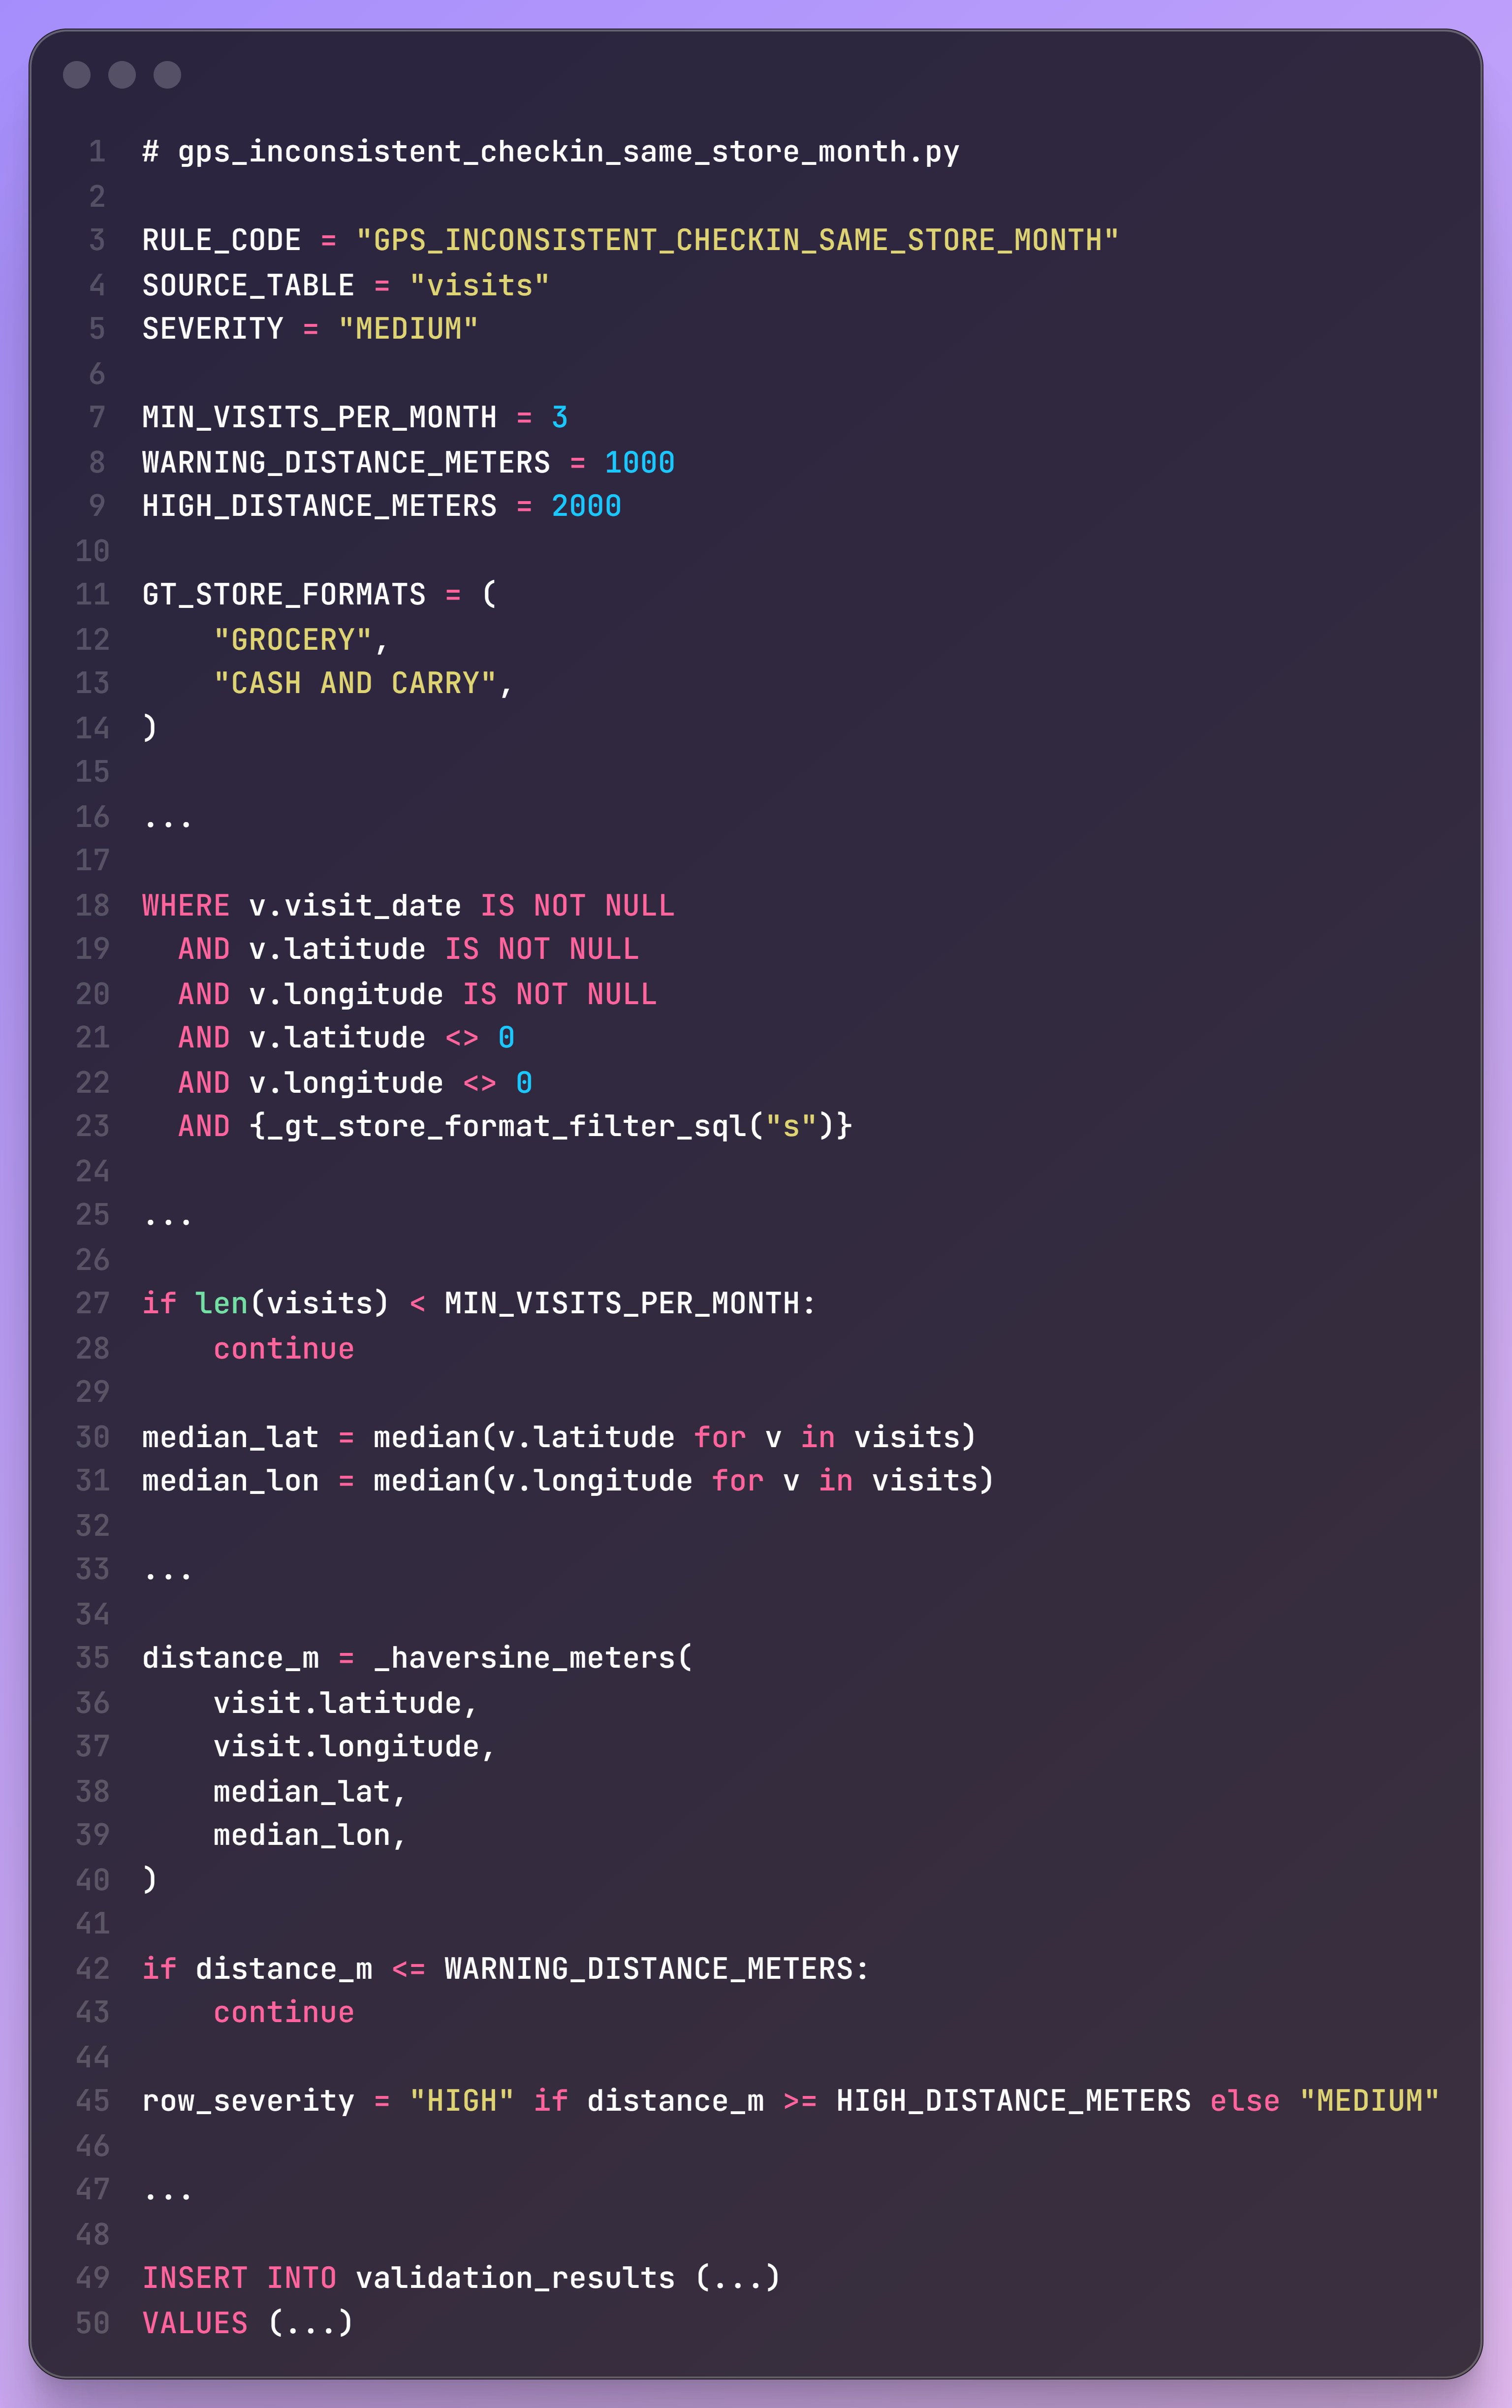
\includegraphics[width=0.60\textwidth]{figures/validation/gps_rule_implementation.png}
\caption{Implémentation de la règle GPS appliquée aux formats GT}
\label{fig:gps_rule_implementation}
\end{figure}

La figure \ref{fig:gps_rule_implementation} montre un extrait du code de la règle GPS. Elle met en évidence le périmètre GT, les seuils de distance, le calcul de la position médiane, la comparaison avec la position observée et l’insertion des résultats dans la table \dbtable{validation\_results}.

\subsection{Traçabilité de l’exécution du moteur}

Au-delà de l’implémentation des règles, le moteur conserve une trace de chaque exécution dans la table \dbtable{validation\_run\_log}. Cette traçabilité permet de vérifier le statut du traitement, le nombre de règles exécutées et le nombre de situations détectées.

\begin{figure}[H]
\centering
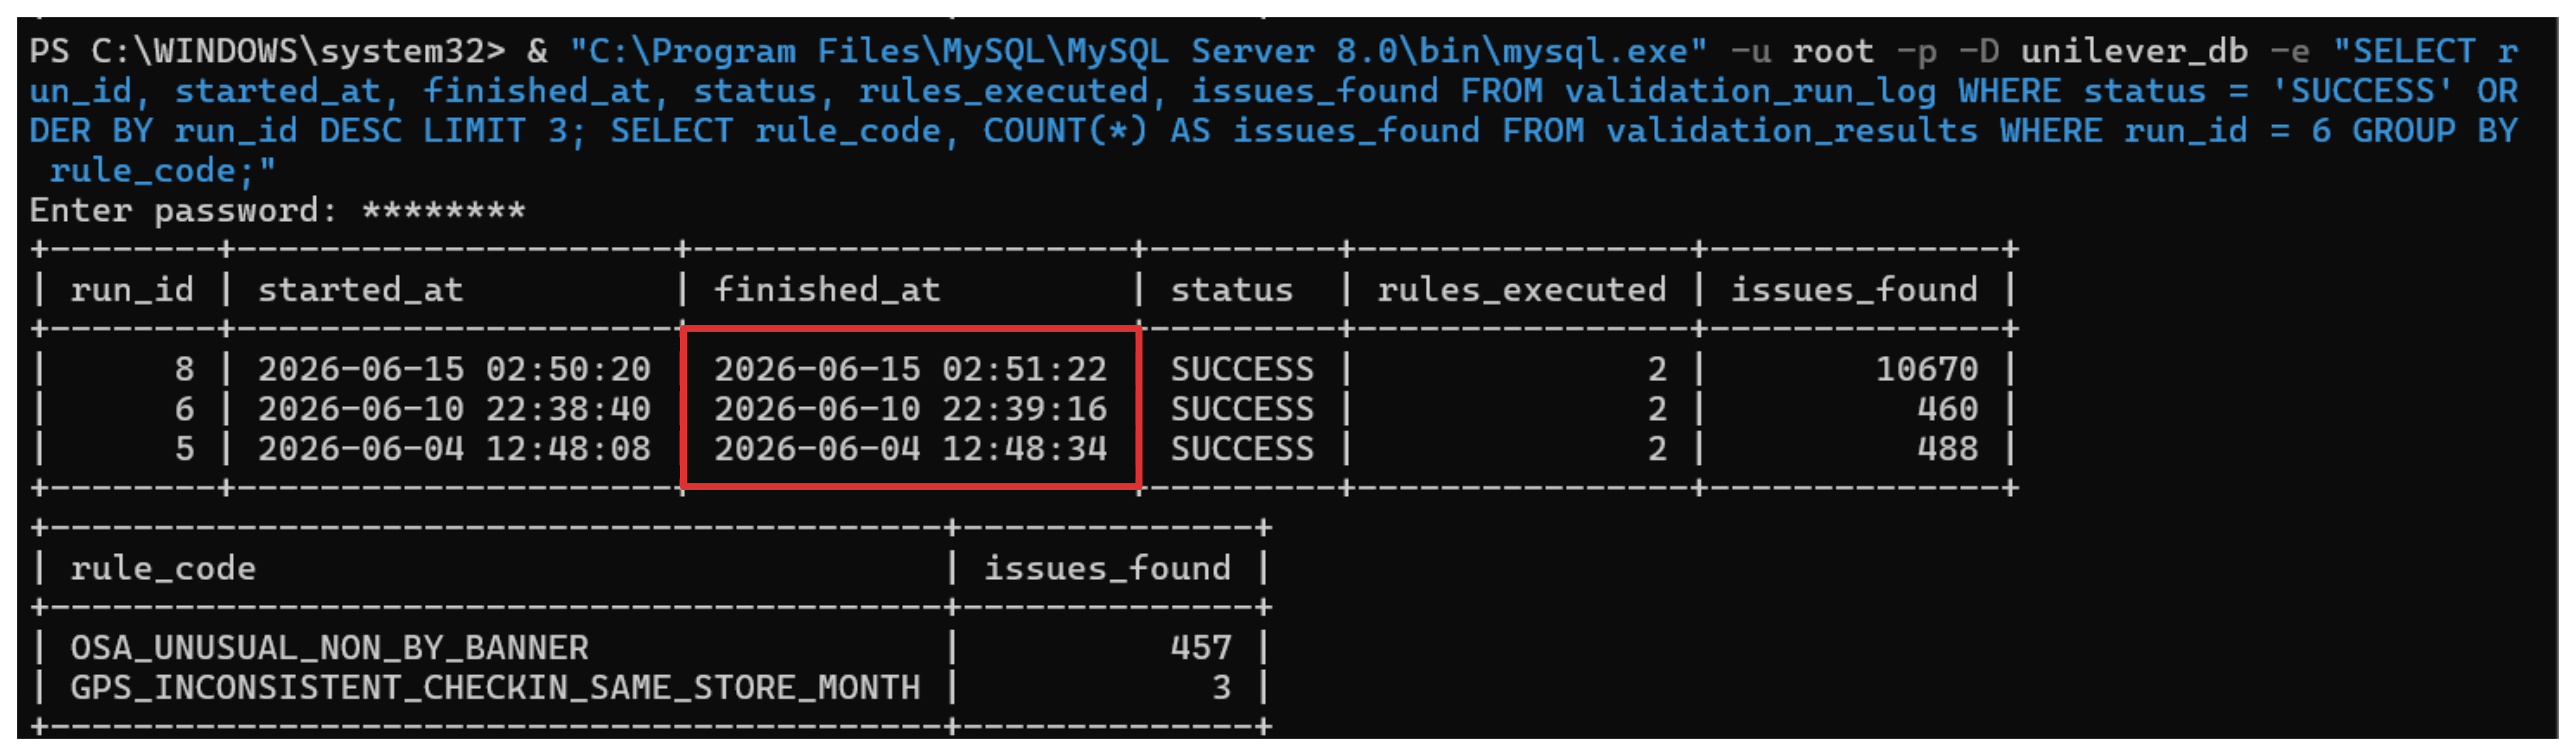
\includegraphics[width=1\textwidth]{figures/validation/validation_execution_terminal.png}
\caption{Résultat d’exécution du moteur de validation}
\label{fig:validation_execution_terminal}
\end{figure}

La figure \ref{fig:validation_execution_terminal} montre un exemple d’exécution réussie du moteur de validation. Elle confirme que les règles ont été exécutées et que les situations détectées ont été enregistrées dans la base MySQL.

\section{Développement de la couche Business Intelligence}

La couche Business Intelligence constitue la partie analytique de la solution. Elle permet d’exploiter les données centralisées dans MySQL afin de construire des vues de pilotage destinées au suivi de l’exécution terrain.

Dans le cadre du projet, Power BI a été utilisé pour préparer une première restitution décisionnelle à partir de la base \dbtable{unilever\_db}. Cette partie présente la préparation technique de la couche BI : connexion à MySQL, structuration du modèle, création des mesures DAX et préparation des vues de restitution \cite{powerbi-doc}.

\subsection{Connexion à la base MySQL}

La préparation de la couche BI commence par une connexion directe entre Power BI et la base MySQL \dbtable{unilever\_db}. Ce choix permet d’exploiter les données déjà centralisées par le pipeline Data Engineering, au lieu de repartir des fichiers Excel bruts.

\begin{figure}[H]
\centering
\begin{minipage}{0.45\textwidth}
\centering
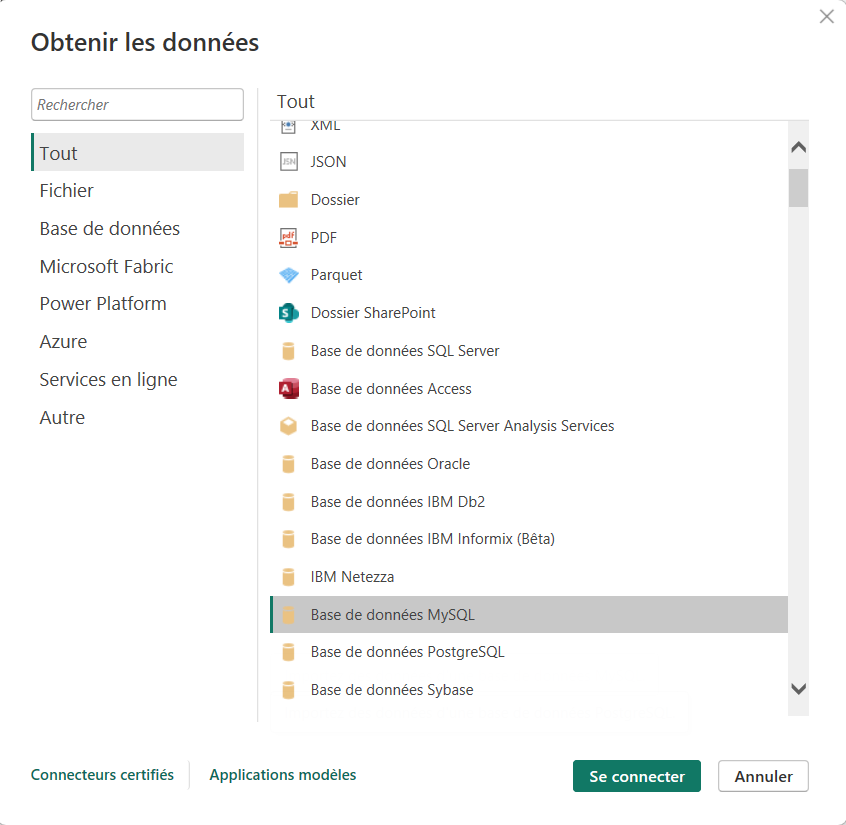
\includegraphics[width=\textwidth]{figures/dashboards/powerbi_mysql_connector.png}
\end{minipage}
\hfill
\begin{minipage}{0.45\textwidth}
\centering
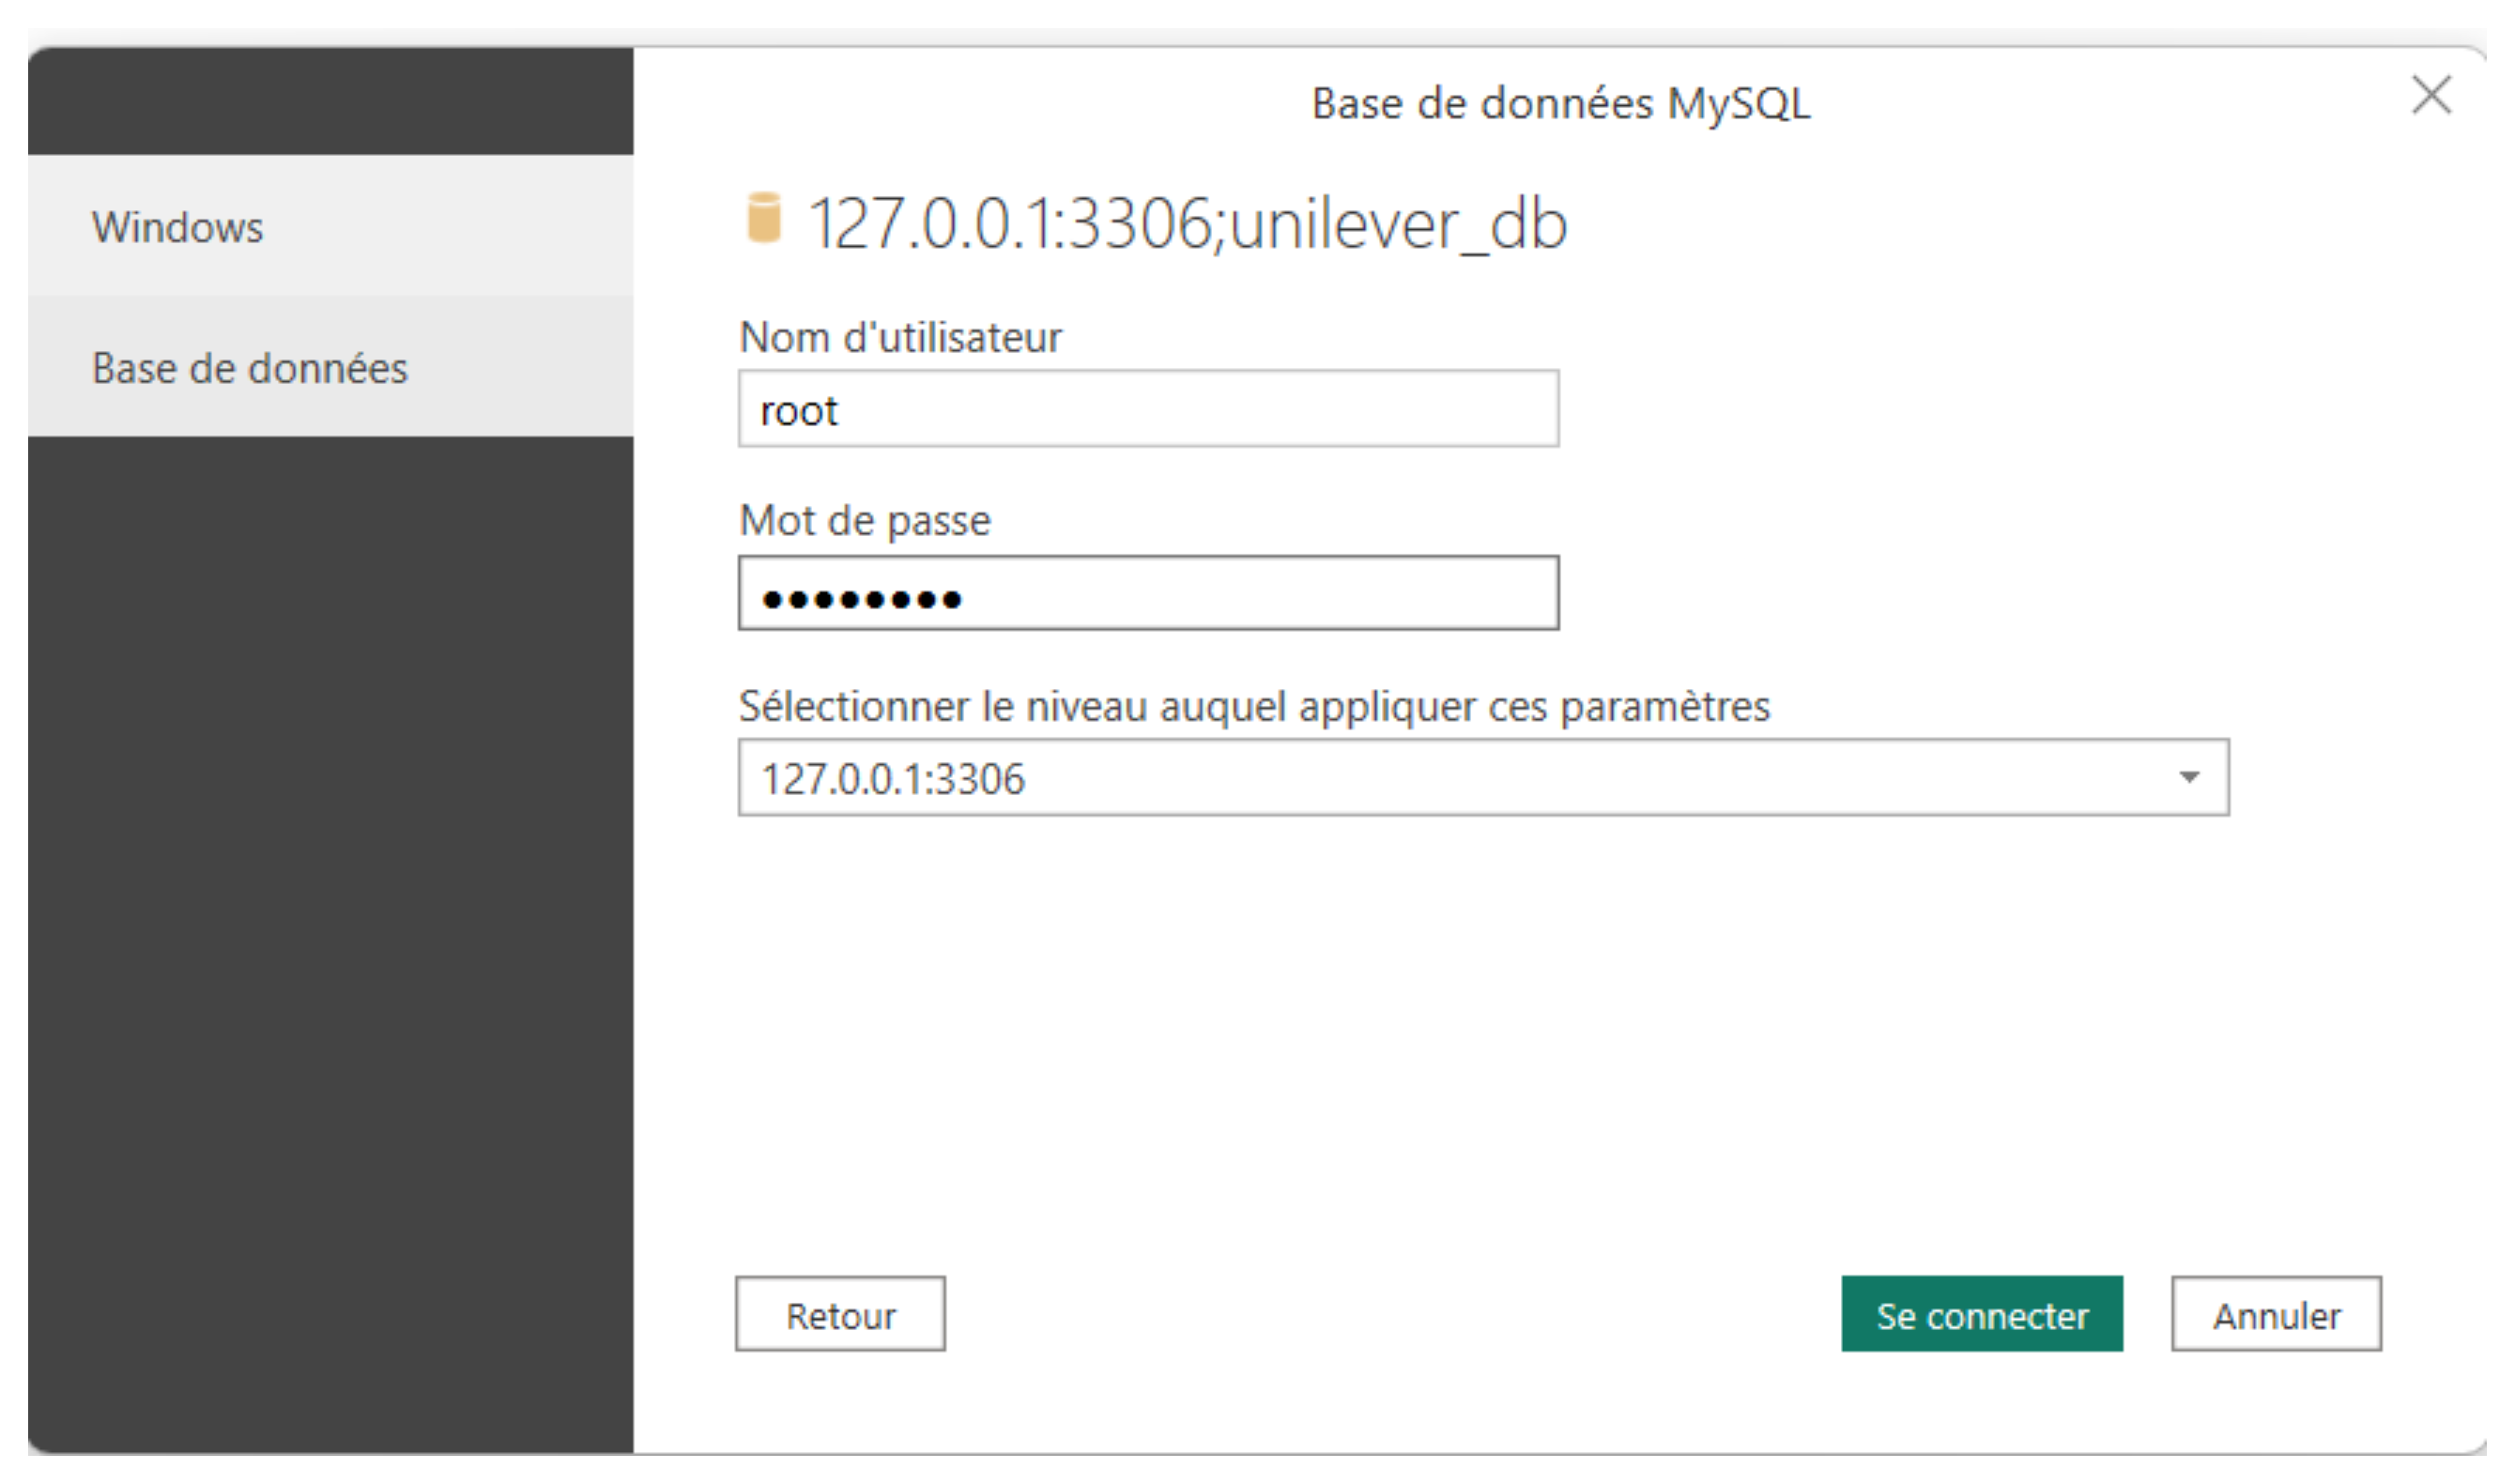
\includegraphics[width=\textwidth]{figures/dashboards/powerbi_mysql_connection.png}
\end{minipage}
\caption{Connexion de Power BI à la base MySQL \dbtable{unilever\_db}}
\label{fig:powerbi_mysql_connection}
\end{figure}

La figure \ref{fig:powerbi_mysql_connection} illustre la sélection du connecteur MySQL et la configuration de la connexion à la base locale. Cette connexion permet d’utiliser MySQL comme source principale du modèle Power BI.

\subsection{Préparation du modèle Power BI}

Après la connexion à MySQL, les tables utiles sont sélectionnées selon les besoins d’analyse. La sélection se concentre principalement sur les données nécessaires au suivi opérationnel : la table \dbtable{fact\_coverage}, les visites, les magasins, les merchandisers, les superviseurs et certaines tables de tâches.

Le modèle Power BI est ensuite structuré à travers les relations nécessaires entre les tables. Cette étape permet d’assurer la cohérence des filtres entre les dates, les merchandisers, les magasins et les données opérationnelles. Les tables de validation restent principalement réservées au portail back-office interne.

\begin{figure}[H]
\centering
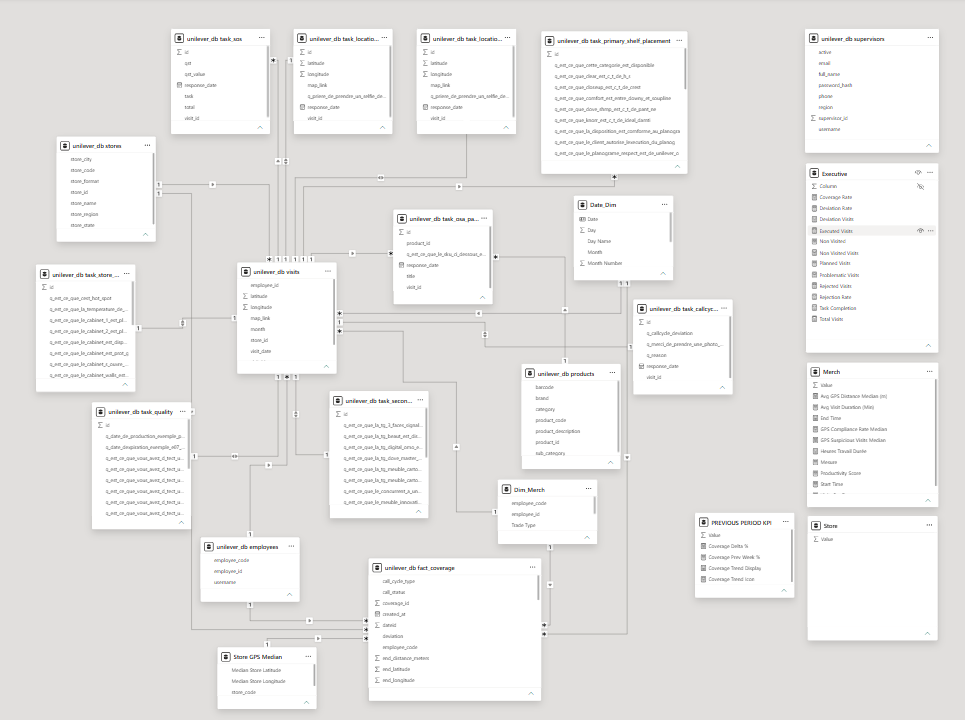
\includegraphics[width=1\textwidth]{figures/dashboards/powerbi_model_relationships.png}
\caption{Modèle relationnel préparé dans Power BI}
\label{fig:powerbi_model_relationships}
\end{figure}

La figure \ref{fig:powerbi_model_relationships} présente le modèle relationnel préparé dans Power BI. Ce modèle permet de passer d’un simple import de tables à une structure exploitable pour le filtrage, l’agrégation et le calcul des indicateurs.

\subsection{Mesures DAX et indicateurs construits}

Plusieurs mesures DAX ont été créées afin de transformer les données opérationnelles en indicateurs dynamiques. Ces mesures permettent de calculer les visites planifiées, les visites exécutées, le taux de couverture, les déviations ainsi qu’un score synthétique de productivité.

La logique de calcul repose principalement sur la table \dbtable{fact\_coverage}. Les mesures se recalculent automatiquement selon les filtres sélectionnés dans Power BI, notamment la période, le merchandiser, le superviseur, la ville ou le format de magasin.

\begin{figure}[H]
\centering
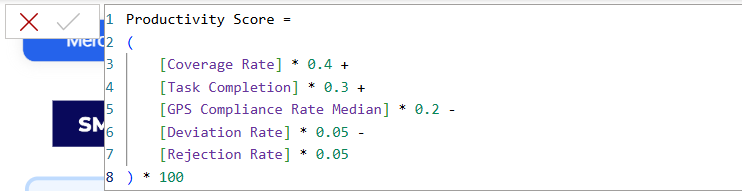
\includegraphics[width=0.82\textwidth]{figures/dashboards/powerbi_dax_productivity_score.png}
\caption{Mesure DAX du score de productivité}
\label{fig:powerbi_dax_productivity_score}
\end{figure}

La figure \ref{fig:powerbi_dax_productivity_score} présente la mesure DAX utilisée pour construire le score de productivité. Ce score synthétise plusieurs dimensions de performance opérationnelle dans un seul indicateur.
\begin{figure}[H]
\centering
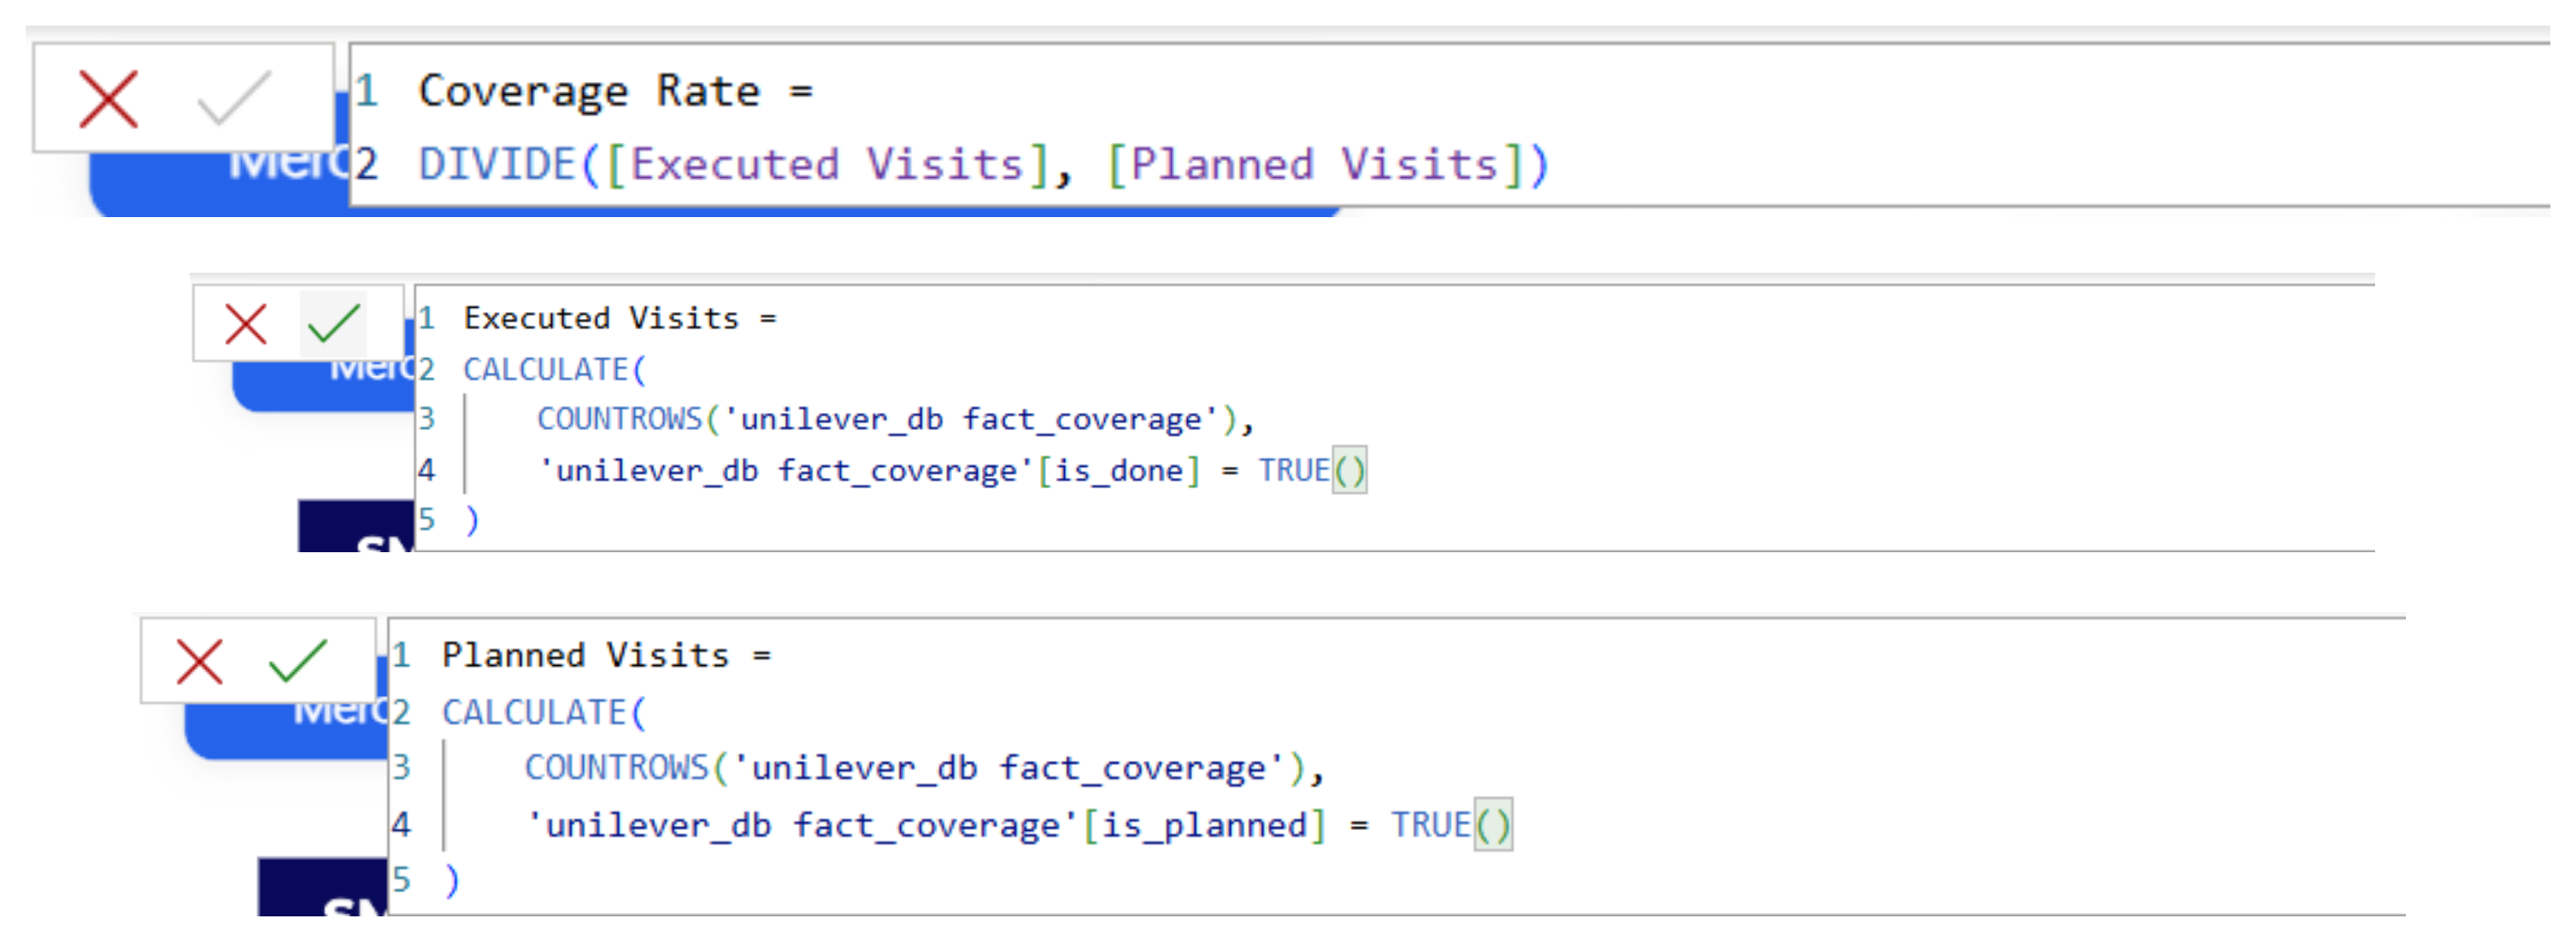
\includegraphics[width=0.95\textwidth]{figures/dashboards/powerbi_dax_coverage_measures.png}
\caption{Exemples de mesures DAX liées au taux de couverture}
\label{fig:powerbi_dax_coverage_measures}
\end{figure}

La figure \ref{fig:powerbi_dax_coverage_measures} présente des exemples de mesures DAX utilisées pour calculer les visites planifiées, les visites exécutées et le taux de couverture. Ces mesures constituent la base des indicateurs opérationnels affichés dans les tableaux de bord.

\subsection{Vues de restitution préparées}

Deux vues principales ont été préparées dans Power BI afin d’exploiter le modèle BI construit à partir de MySQL. La première vue, intitulée \textit{National Retail Execution Dashboard}, est conçue comme une vue de pilotage globale de l’exécution terrain.

La seconde vue, intitulée \textit{Merchandiser Performance Intelligence}, est orientée vers l’analyse individuelle des merchandisers. Elle permet de structurer le suivi autour de la couverture, de la complétion des tâches, de la durée de visite et des indicateurs liés à la cohérence GPS.

Dans ce chapitre, la couche BI est présentée sous l’angle de sa préparation technique. Les captures finales des tableaux de bord et l’interprétation des résultats seront présentées dans le chapitre consacré à la réalisation, aux tests et aux résultats.

\section{Développement de la couche backend}

La couche backend constitue l’intermédiaire entre la base MySQL \dbtable{unilever\_db} et les interfaces applicatives de la solution. Elle a été développée avec Spring Boot afin d’exposer les données centralisées sous forme d’APIs REST consommées par l’application mobile et par le portail back-office \cite{springboot-doc}.

Cette couche ne se limite pas à transmettre les données brutes. Elle applique également une partie de la logique métier nécessaire à l’exploitation de la solution, notamment le filtrage par superviseur, le calcul des indicateurs opérationnels et la séparation entre les données accessibles côté client et les résultats de validation réservés au back-office interne.

\subsection{Rôle de la couche backend}

Le rôle principal du backend est de rendre les données préparées par le pipeline Data Engineering accessibles à travers des services applicatifs contrôlés. Les tables MySQL contiennent les données issues du \textit{Data Dump}, du \textit{Coverage} et du moteur de validation, mais elles ne sont pas exploitées directement par les interfaces.

Le backend organise donc les accès selon les usages. L’application mobile est orientée vers la consultation client : elle affiche les magasins affectés, les statuts d’exécution et les indicateurs opérationnels. À l’inverse, le portail back-office est réservé au suivi interne des situations détectées par les règles de validation.

Cette séparation permet de distinguer clairement les APIs destinées à la consultation mobile et celles destinées au suivi interne des validations.

\subsection{Organisation technique du backend}

Le backend repose sur une organisation en contrôleurs REST, services métier et objets de transfert de données. Les contrôleurs exposent les endpoints, les services portent la logique de traitement et les DTOs structurent les réponses retournées aux interfaces sous forme JSON.

L’accès aux données est réalisé à l’aide de \dbtable{JdbcTemplate}. Ce choix permet de garder un contrôle direct sur les requêtes SQL utilisées pour interroger les tables opérationnelles et les tables de validation, notamment pour les agrégations, les filtres par période et les jointures entre tables.

\begin{figure}[H]
\centering
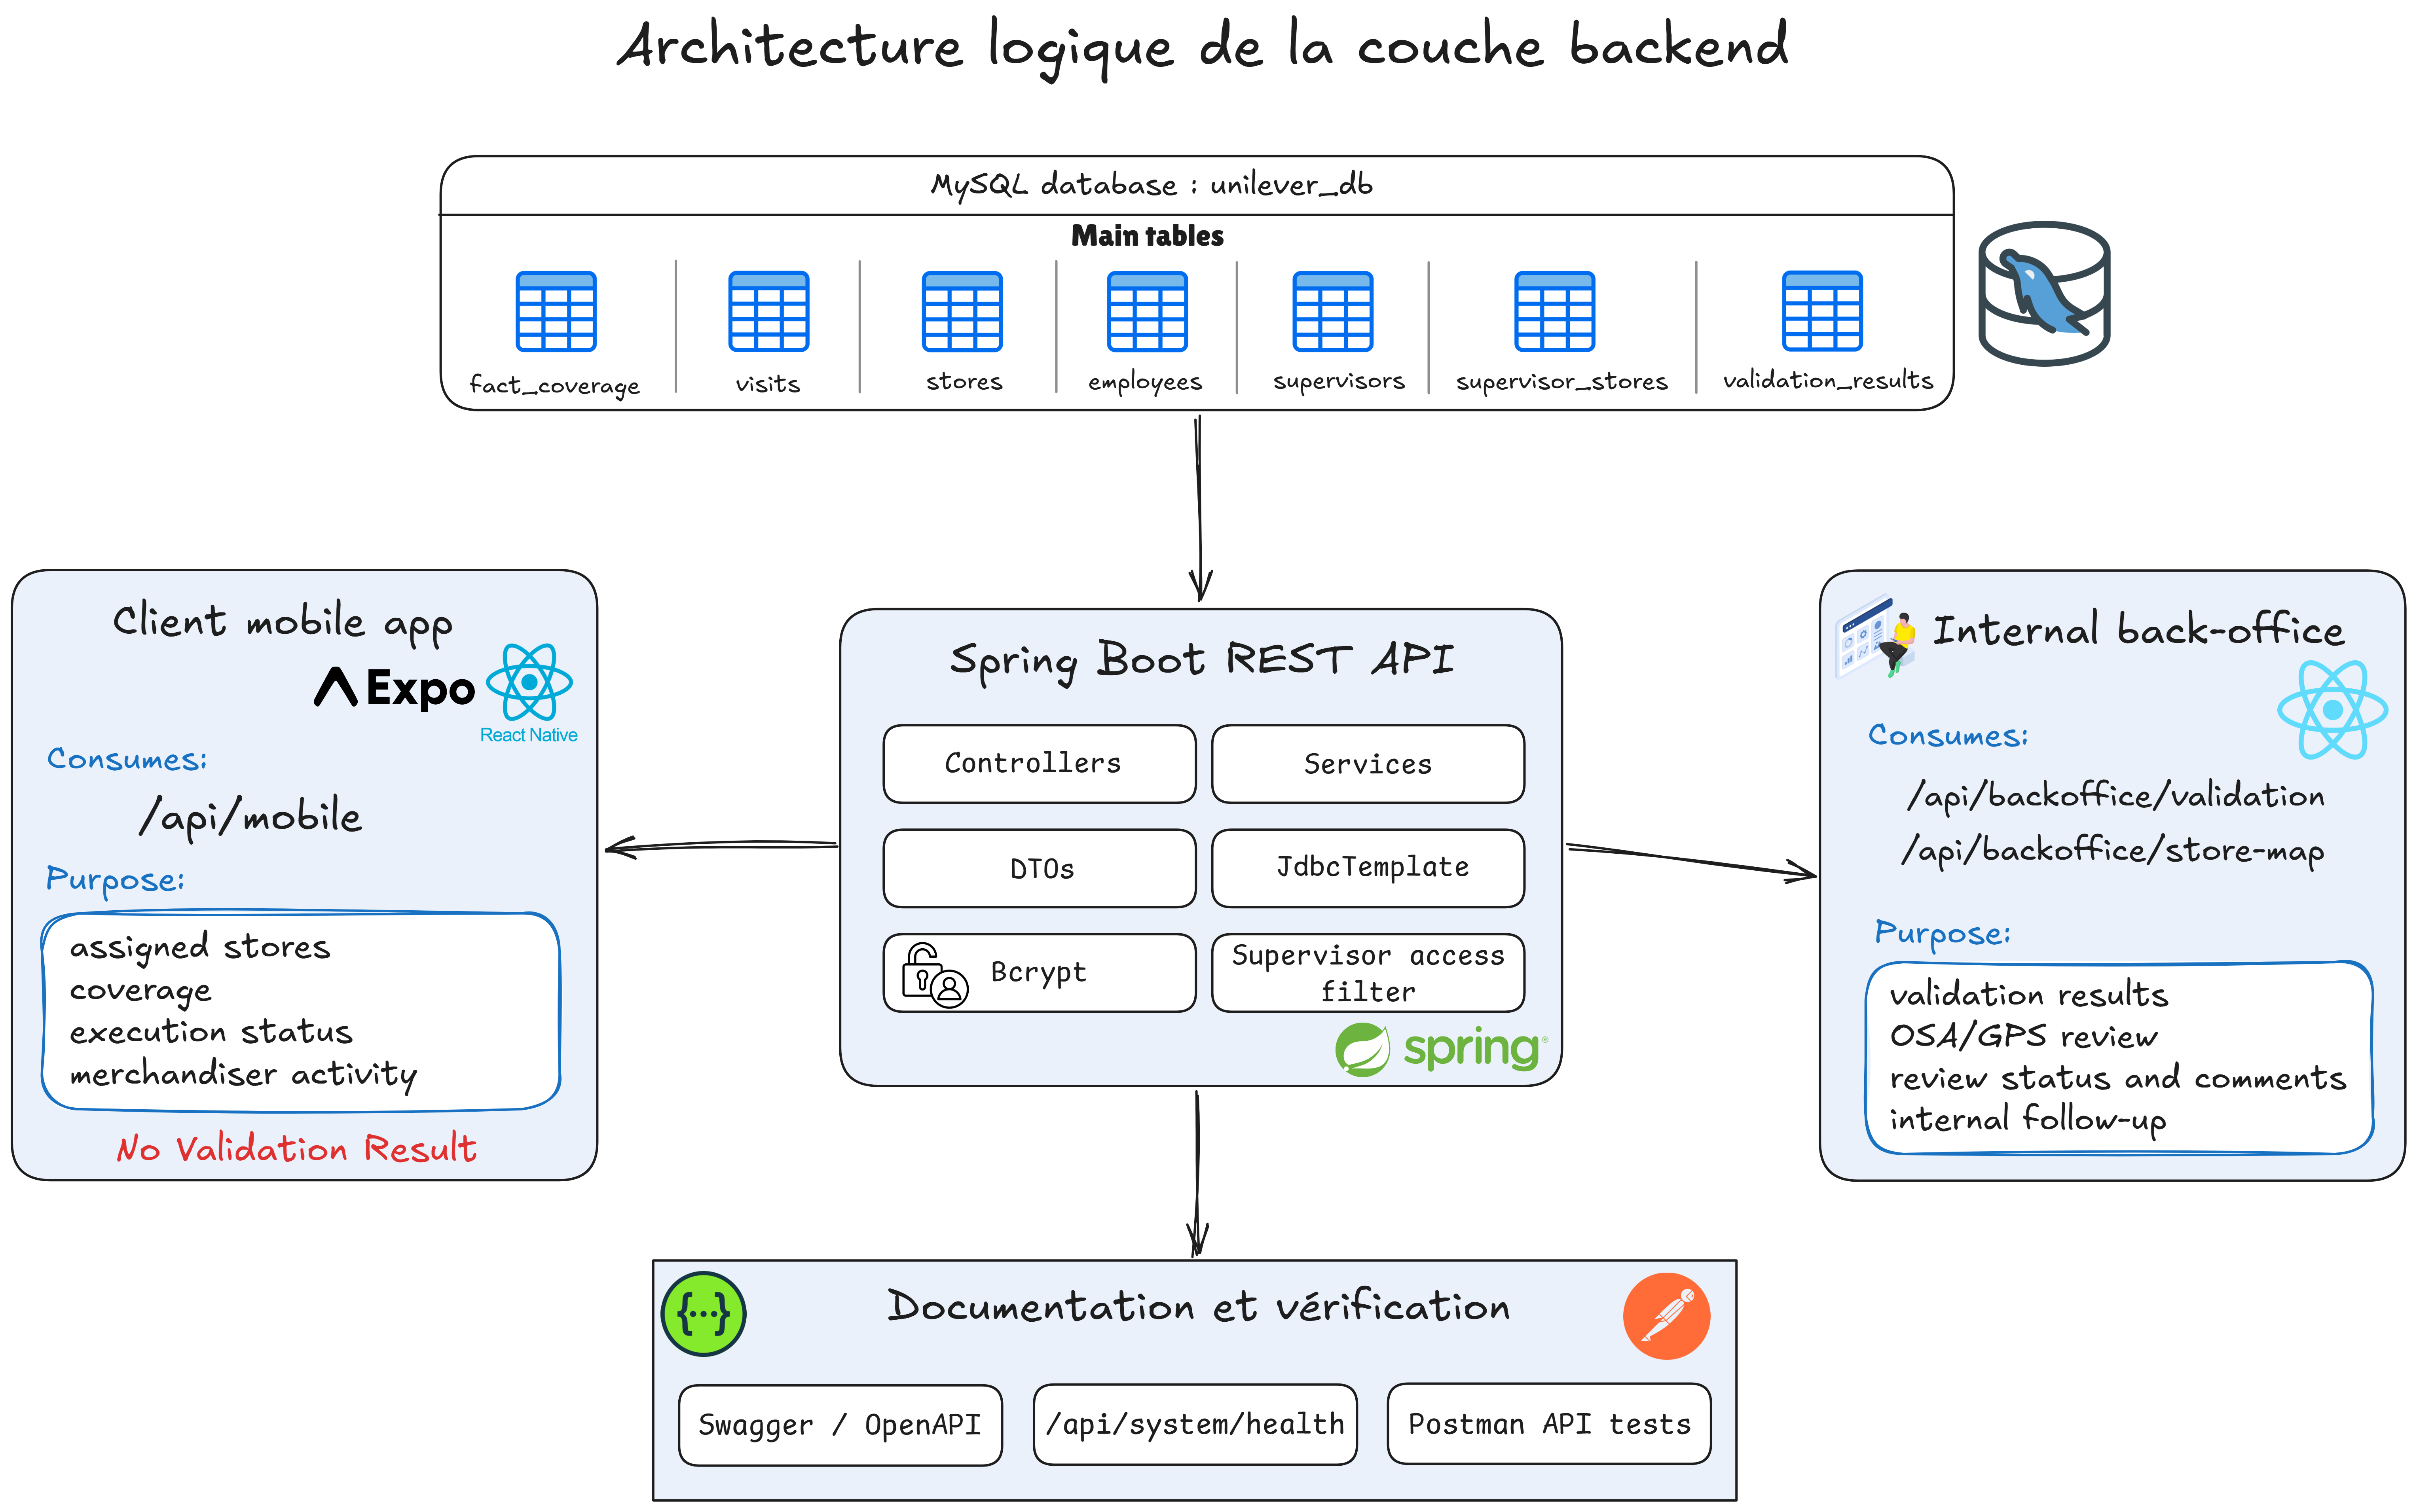
\includegraphics[width=1\textwidth]{figures/API/backend_logical_architecture.png}
\caption{Architecture logique de la couche backend}
\label{fig:backend_logical_architecture}
\end{figure}

La figure \ref{fig:backend_logical_architecture} présente l’architecture logique de la couche backend. Elle met en évidence le rôle central de l’API Spring Boot entre la base MySQL, l’application mobile, le portail back-office et les outils de documentation et de vérification.

\subsection{Gestion de l’accès mobile par superviseur}

L’accès mobile a été conçu de manière ciblée afin que chaque superviseur consulte uniquement les magasins relevant de son périmètre. Cette logique repose sur les tables \dbtable{supervisors} et \dbtable{supervisor\_stores}, qui permettent d’associer chaque superviseur à un ensemble de magasins autorisés.

Dans la base MySQL, chaque superviseur est identifié par un code, un nom, une ville et une région. La table d’association permet ensuite de définir le nombre de magasins rattachés à ce superviseur. Cette organisation constitue la base du filtrage appliqué dans l’application mobile lors de la consultation des magasins.

\begin{figure}[H]
    \centering
    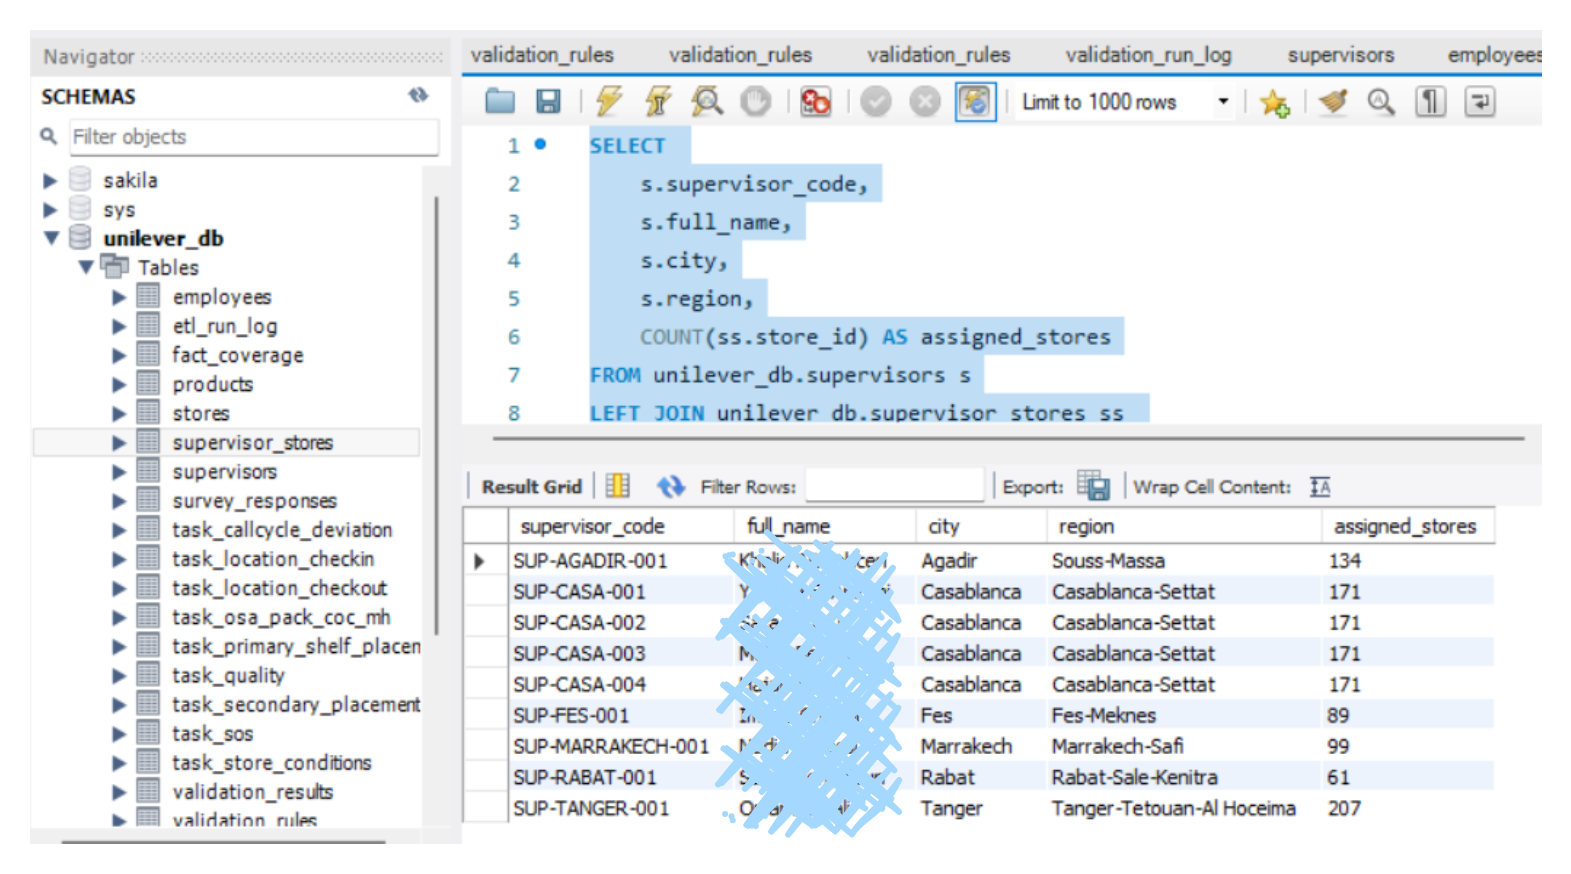
\includegraphics[width=0.95\textwidth]{figures/database/supervisor_store_assignment.png}
    \caption{Exemple de gestion du périmètre d’accès mobile par superviseur dans MySQL}
    \label{fig:supervisor_store_assignment}
\end{figure}

La figure \ref{fig:supervisor_store_assignment} montre un exemple de requête permettant de vérifier l’affectation des magasins par superviseur. Cette vérification confirme que l’accès mobile peut être limité à un périmètre précis, en fonction des magasins associés à chaque superviseur.

\subsection{Logique d’authentification mobile}

La logique d’authentification mobile repose sur une connexion par email et mot de passe. Lorsqu’un utilisateur saisit ses identifiants dans l’application mobile, une requête est envoyée vers l’endpoint \dbtable{/api/mobile/login}. Le backend vérifie l’existence d’un compte actif, puis compare le mot de passe saisi avec le hachage stocké dans la base à l’aide de BCrypt.

Après une authentification réussie, le backend retourne les informations du superviseur connecté, notamment son identifiant, son rôle et le nombre de magasins affectés. Ces informations permettent ensuite à l’application mobile de charger uniquement les données correspondant au périmètre autorisé.

\subsection{Séparation entre consultation client et validation interne}

L’architecture applicative repose sur une séparation claire entre les services destinés à la consultation client et ceux réservés au suivi interne. Les endpoints mobiles permettent d’alimenter l’application de consultation utilisée par les superviseurs côté client, tandis que les endpoints back-office sont dédiés au traitement des situations détectées par le moteur de validation.

Cette séparation permet d’éviter l’exposition directe des résultats de validation dans l’application mobile. Les superviseurs accèdent uniquement aux informations utiles à la consultation opérationnelle, alors que les équipes internes disposent d’un portail spécifique pour analyser les anomalies, consulter leur détail et suivre leur traitement.

\begin{figure}[H]
    \centering
    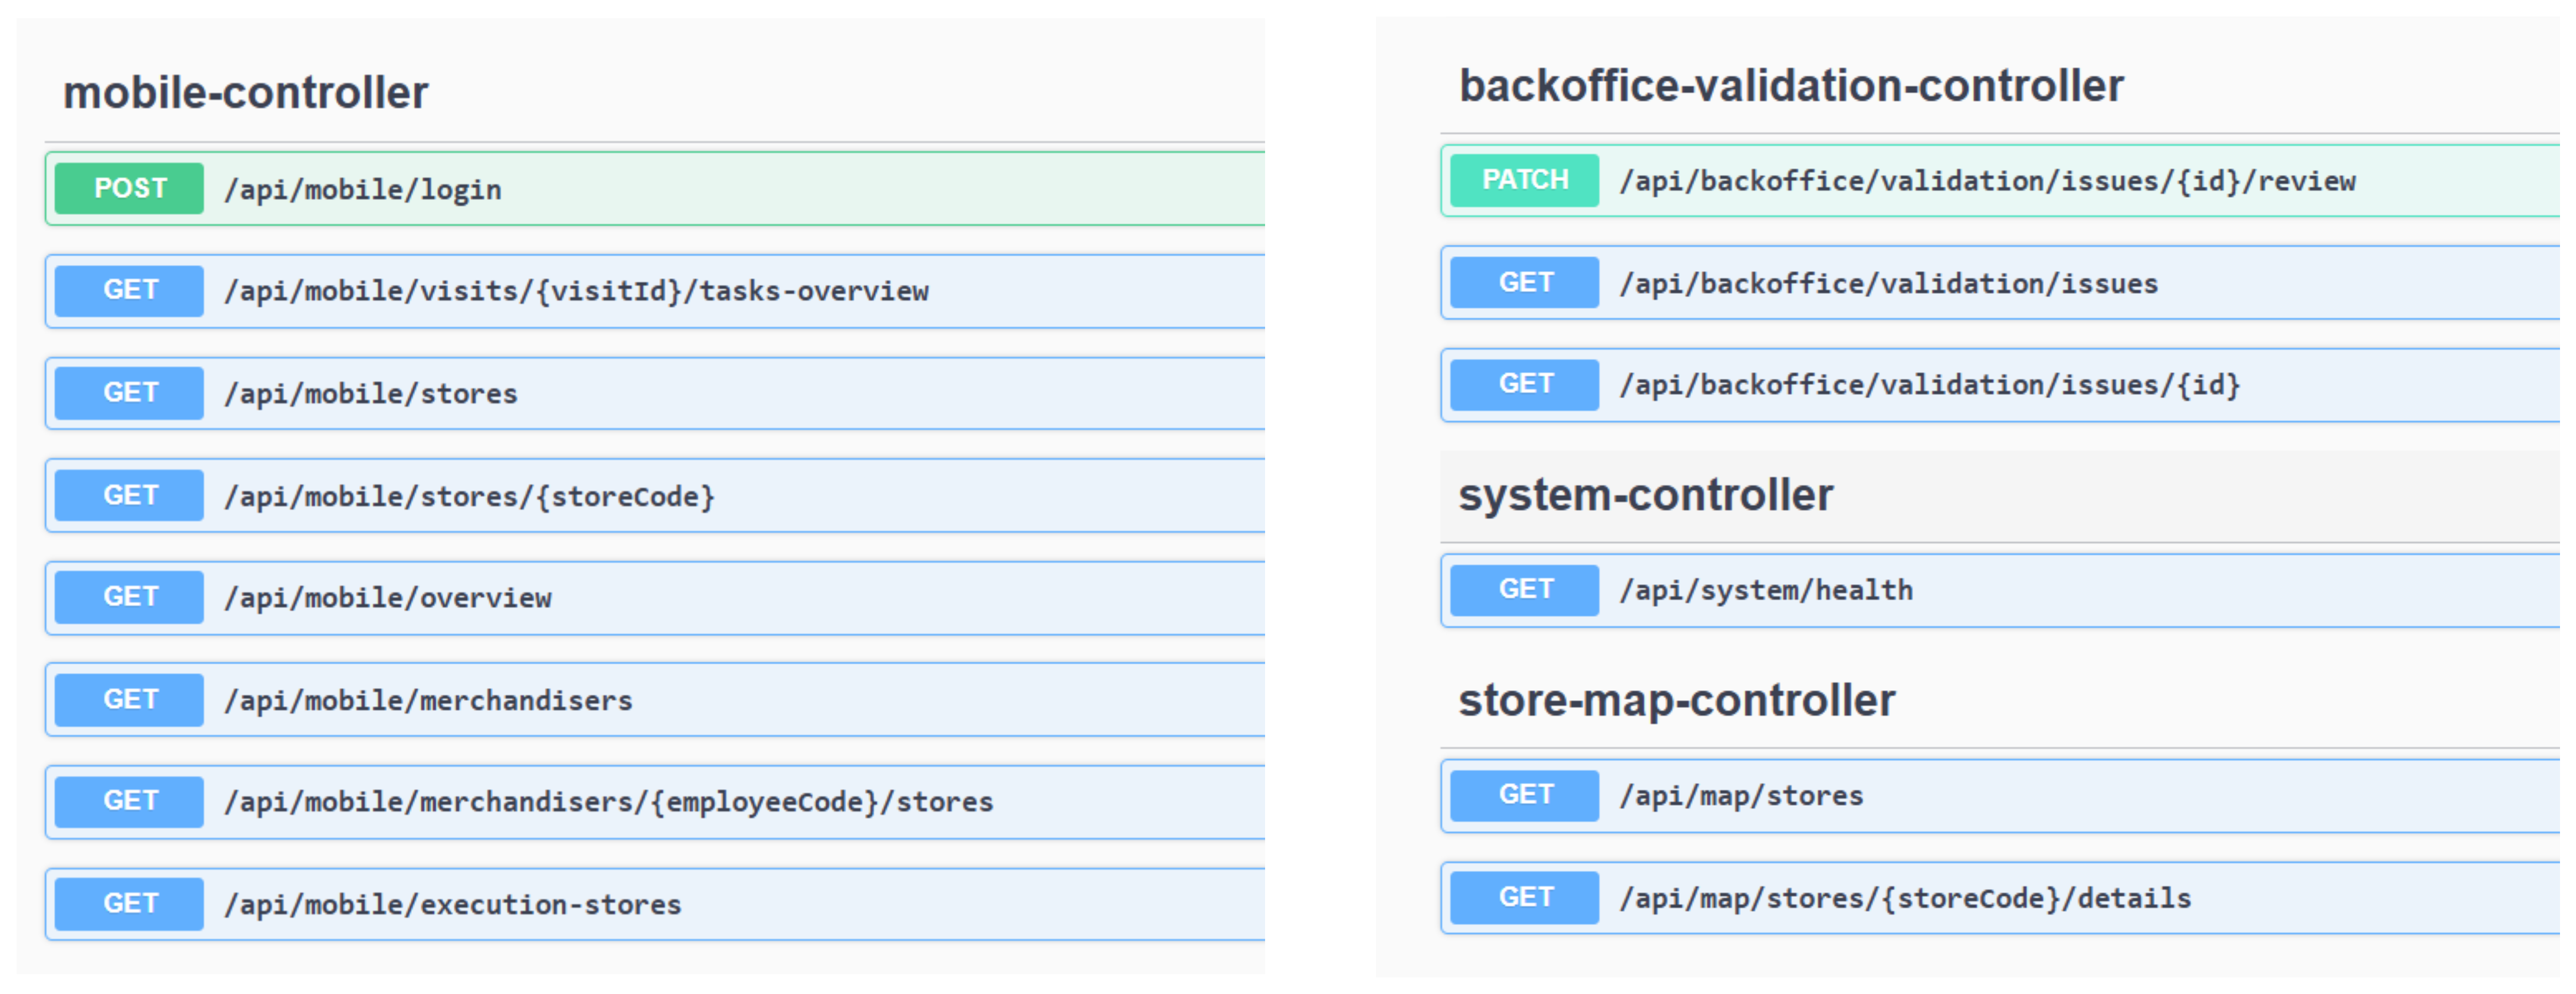
\includegraphics[width=0.80\textwidth]{figures/API/swagger_api_groups.png}
    \caption{Documentation Swagger des endpoints mobiles et back-office}
    \label{fig:swagger_api_groups}
\end{figure}

La figure \ref{fig:swagger_api_groups} illustre cette séparation à travers la documentation Swagger. On y distingue les endpoints mobiles destinés à la consultation client, les endpoints back-office liés aux validations, les services cartographiques ainsi que l’endpoint système utilisé pour vérifier l’état du backend.

\subsection{Vérification des APIs}

Afin de vérifier le bon fonctionnement des services exposés par le backend, Postman a été utilisé pour tester certains endpoints. Un premier test a été réalisé sur l’authentification mobile afin de confirmer que l’API reçoit correctement l’email et le mot de passe, puis retourne les informations du superviseur connecté lorsque les identifiants sont valides.

\begin{figure}[H]
\centering
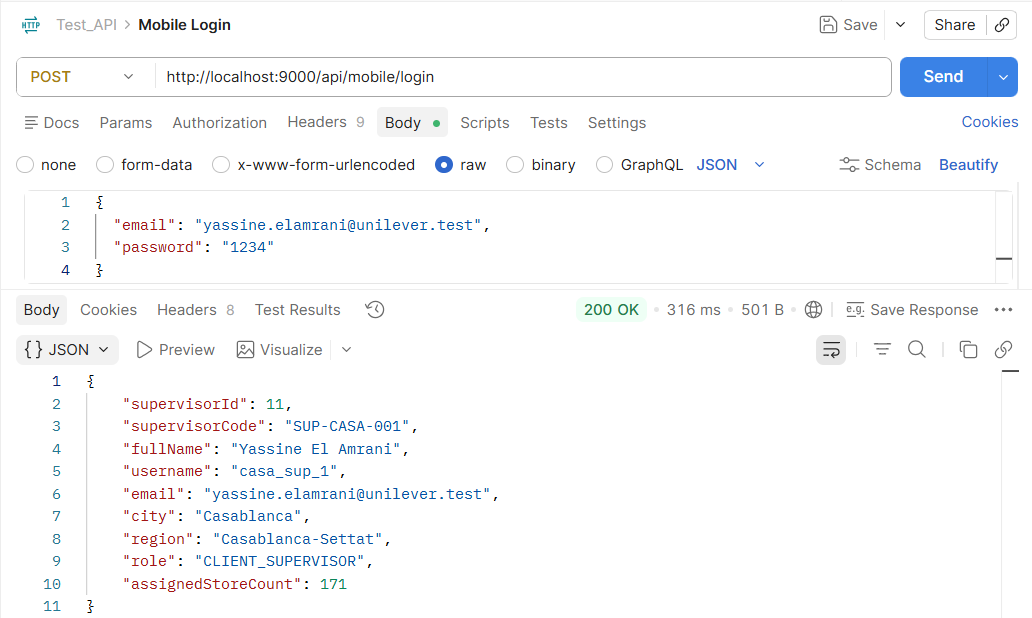
\includegraphics[width=0.85\textwidth]{figures/API/postman_mobile_login.png}
\caption{Test de l’authentification mobile par email avec Postman}
\label{fig:postman_mobile_login}
\end{figure}

La figure \ref{fig:postman_mobile_login} montre un appel réussi à l’endpoint \dbtable{/api/mobile/login}. La présence du champ \dbtable{assignedStoreCount} confirme que l’authentification est liée au périmètre de magasins affectés au superviseur.

Une seconde vérification a été réalisée sur l’endpoint \dbtable{/api/system/health}. Cet endpoint permet de contrôler rapidement l’état du backend et sa connexion à la base MySQL.

\begin{figure}[H]
\centering
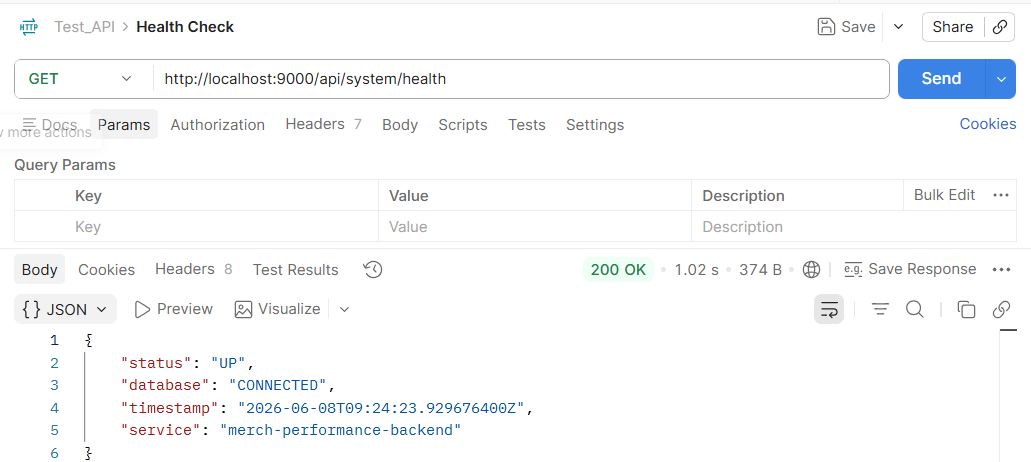
\includegraphics[width=0.85\textwidth]{figures/API/api_system_health.png}
\caption{Vérification de l’état du backend avec l’endpoint \dbtable{/api/system/health}}
\label{fig:api_system_health}
\end{figure}

La figure \ref{fig:api_system_health} confirme que le service backend répond correctement et que la connexion à la base MySQL est opérationnelle. Ces tests complètent la documentation Swagger et permettent de vérifier le bon fonctionnement des principaux services exposés.

\newpage

\section{Développement des interfaces applicatives}

Après la mise en place de la couche backend, la solution a été complétée par deux interfaces applicatives consommant les APIs REST développées. La première est une application mobile de consultation, destinée au suivi opérationnel des magasins affectés. La seconde est un portail back-office interne, destiné à l’exploitation et au suivi des résultats de validation.

Cette séparation permet d’adapter chaque interface à son usage : consultation opérationnelle côté client et suivi interne côté Smollan.

\subsection{Organisation générale des interfaces}

L’organisation des interfaces repose sur deux parcours complémentaires. L’application mobile, développée avec Expo et React Native, consomme principalement les APIs \url{/api/mobile} \cite{expo-doc,reactnative-doc}. Elle regroupe les vues nécessaires à la consultation du périmètre affecté : connexion, tableau de bord, exécution des merchandisers, liste ou carte des magasins et détail magasin.

Le portail back-office, développé avec React, consomme les APIs internes liées aux validations et au suivi cartographique \cite{react-doc}. Il regroupe les vues nécessaires au traitement interne : centre de validation, liste des situations détectées, détail d’une situation, statut de revue, commentaires et suivi cartographique.

\begin{figure}[H]
\centering
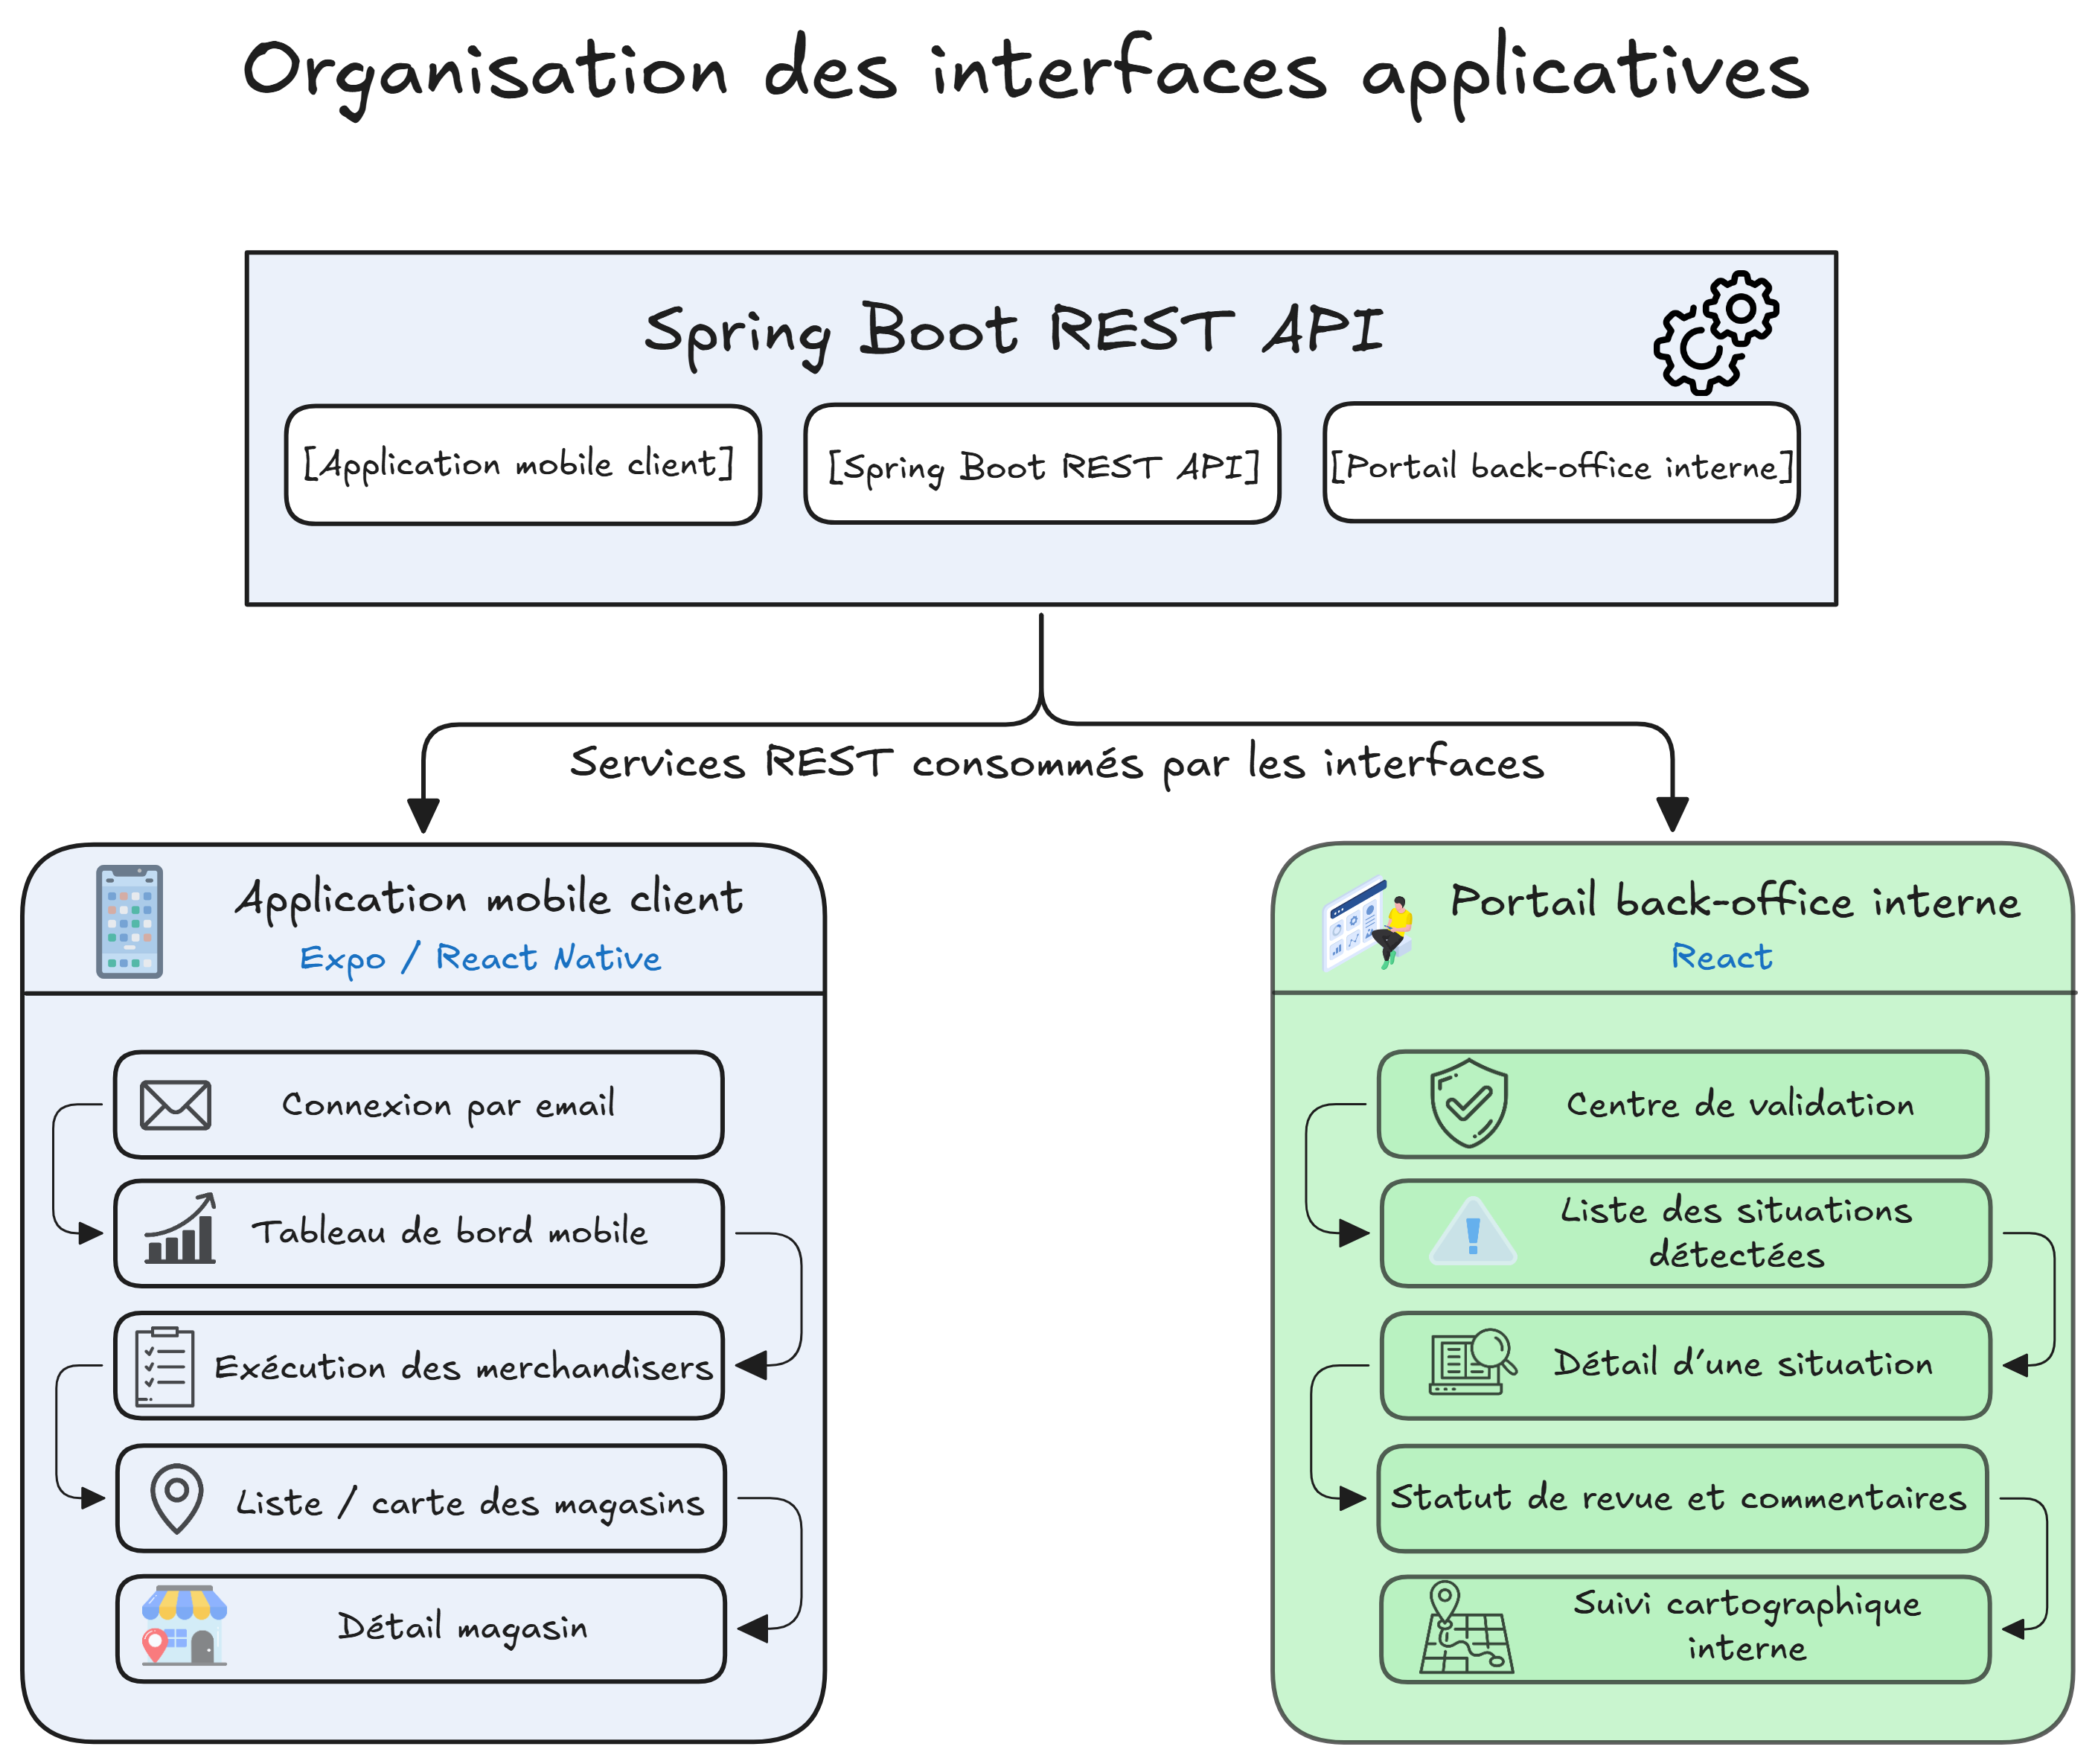
\includegraphics[width=0.9\textwidth]{figures/mobile/interfaces_organization.png}
\caption{Organisation générale des interfaces applicatives}
\label{fig:interfaces_organization}
\end{figure}

La figure \ref{fig:interfaces_organization} présente la séparation entre l’application mobile client et le portail back-office interne, tous deux reliés à la couche backend selon leurs besoins fonctionnels.

\subsection{Application mobile de consultation client}

L’application mobile constitue l’interface de consultation destinée au suivi opérationnel côté client. Elle permet à un superviseur ou commercial connecté de consulter uniquement les magasins associés à son périmètre d’affectation.

Après authentification, l’application récupère les informations du compte connecté puis interroge les endpoints mobiles pour afficher les indicateurs de suivi, l’activité des merchandisers et la liste des magasins. Elle permet également de consulter le détail d’un point de vente, notamment son statut de visite, le merchandiser associé et les informations d’exécution disponibles.

L’application mobile ne présente pas les résultats du moteur de validation. Elle reste orientée vers une consultation opérationnelle claire des magasins, des statuts d’exécution et de l’activité terrain.

\subsection{Portail back-office interne}

Le portail back-office constitue l’interface interne de suivi des situations détectées par le moteur de validation. Contrairement à l’application mobile, il est destiné aux équipes internes Smollan afin de consulter, analyser et suivre les résultats issus des règles de contrôle.

Le back-office consomme principalement les APIs \dbtable{/api/backoffice/validation} et \dbtable{/api/backoffice/store-map}. Il permet d’accéder au centre de validation, à la liste des situations détectées, au détail d’une situation, aux statuts de revue et aux commentaires internes.

Cette interface complète le moteur de validation en transformant les situations détectées automatiquement en éléments de suivi opérationnel. Elle ne remplace pas l’analyse métier, mais facilite l’identification, la revue et le traitement des cas nécessitant une attention.

\subsection{Limites actuelles et évolutions possibles}

Les interfaces développées permettent de valider les principaux usages attendus dans le cadre du projet : consultation mobile du périmètre affecté, suivi opérationnel de l’exécution terrain et revue interne des situations détectées.

Certaines limites restent toutefois à prendre en compte. Le mécanisme d’authentification repose actuellement sur une connexion par email et mot de passe avec hachage BCrypt, sans gestion complète de jetons ou de sessions. De plus, la liste des superviseurs et des magasins affectés repose sur une structure prototype, en attendant la liste officielle du client Unilever.

Les évolutions possibles concernent donc le renforcement de l’authentification, l’intégration de la liste officielle des affectations, l’ajout de filtres avancés et l’enrichissement du portail back-office par des exports ou des indicateurs de synthèse supplémentaires.

\section{Conclusion}

Ce chapitre a présenté la mise en œuvre technique de la solution adoptée, depuis l’ingestion des fichiers \textit{Data Dump} et \textit{Coverage} jusqu’à leur exploitation dans les différentes couches de la solution. Le pipeline Data Engineering a permis de transformer les exports Excel en données structurées dans la base MySQL \dbtable{unilever\_db}, tout en assurant la traçabilité des traitements.

Cette base centralisée alimente ensuite les principales composantes de la solution : le moteur de validation, la couche Business Intelligence, le backend Spring Boot et les interfaces applicatives. Le moteur de validation intègre des contrôles métier OSA pour les formats MT et GPS pour les formats GT. La couche BI prépare les indicateurs de pilotage dans Power BI, tandis que le backend expose les données à travers des APIs REST documentées et vérifiées.

Enfin, les interfaces applicatives ont été organisées selon deux usages distincts : une application mobile dédiée à la consultation opérationnelle du périmètre affecté, et un portail back-office réservé au suivi interne des situations détectées. Le chapitre suivant présentera les tests réalisés ainsi que les principaux résultats obtenus.